\section{Chang'E-4 and Lunar Lander Neutron and Dosimetry Experiment}
\label{sec:change_4_LND}

\subsection{Overview and current status (2019 - 2022)}

\begin{figure}
    \centering
    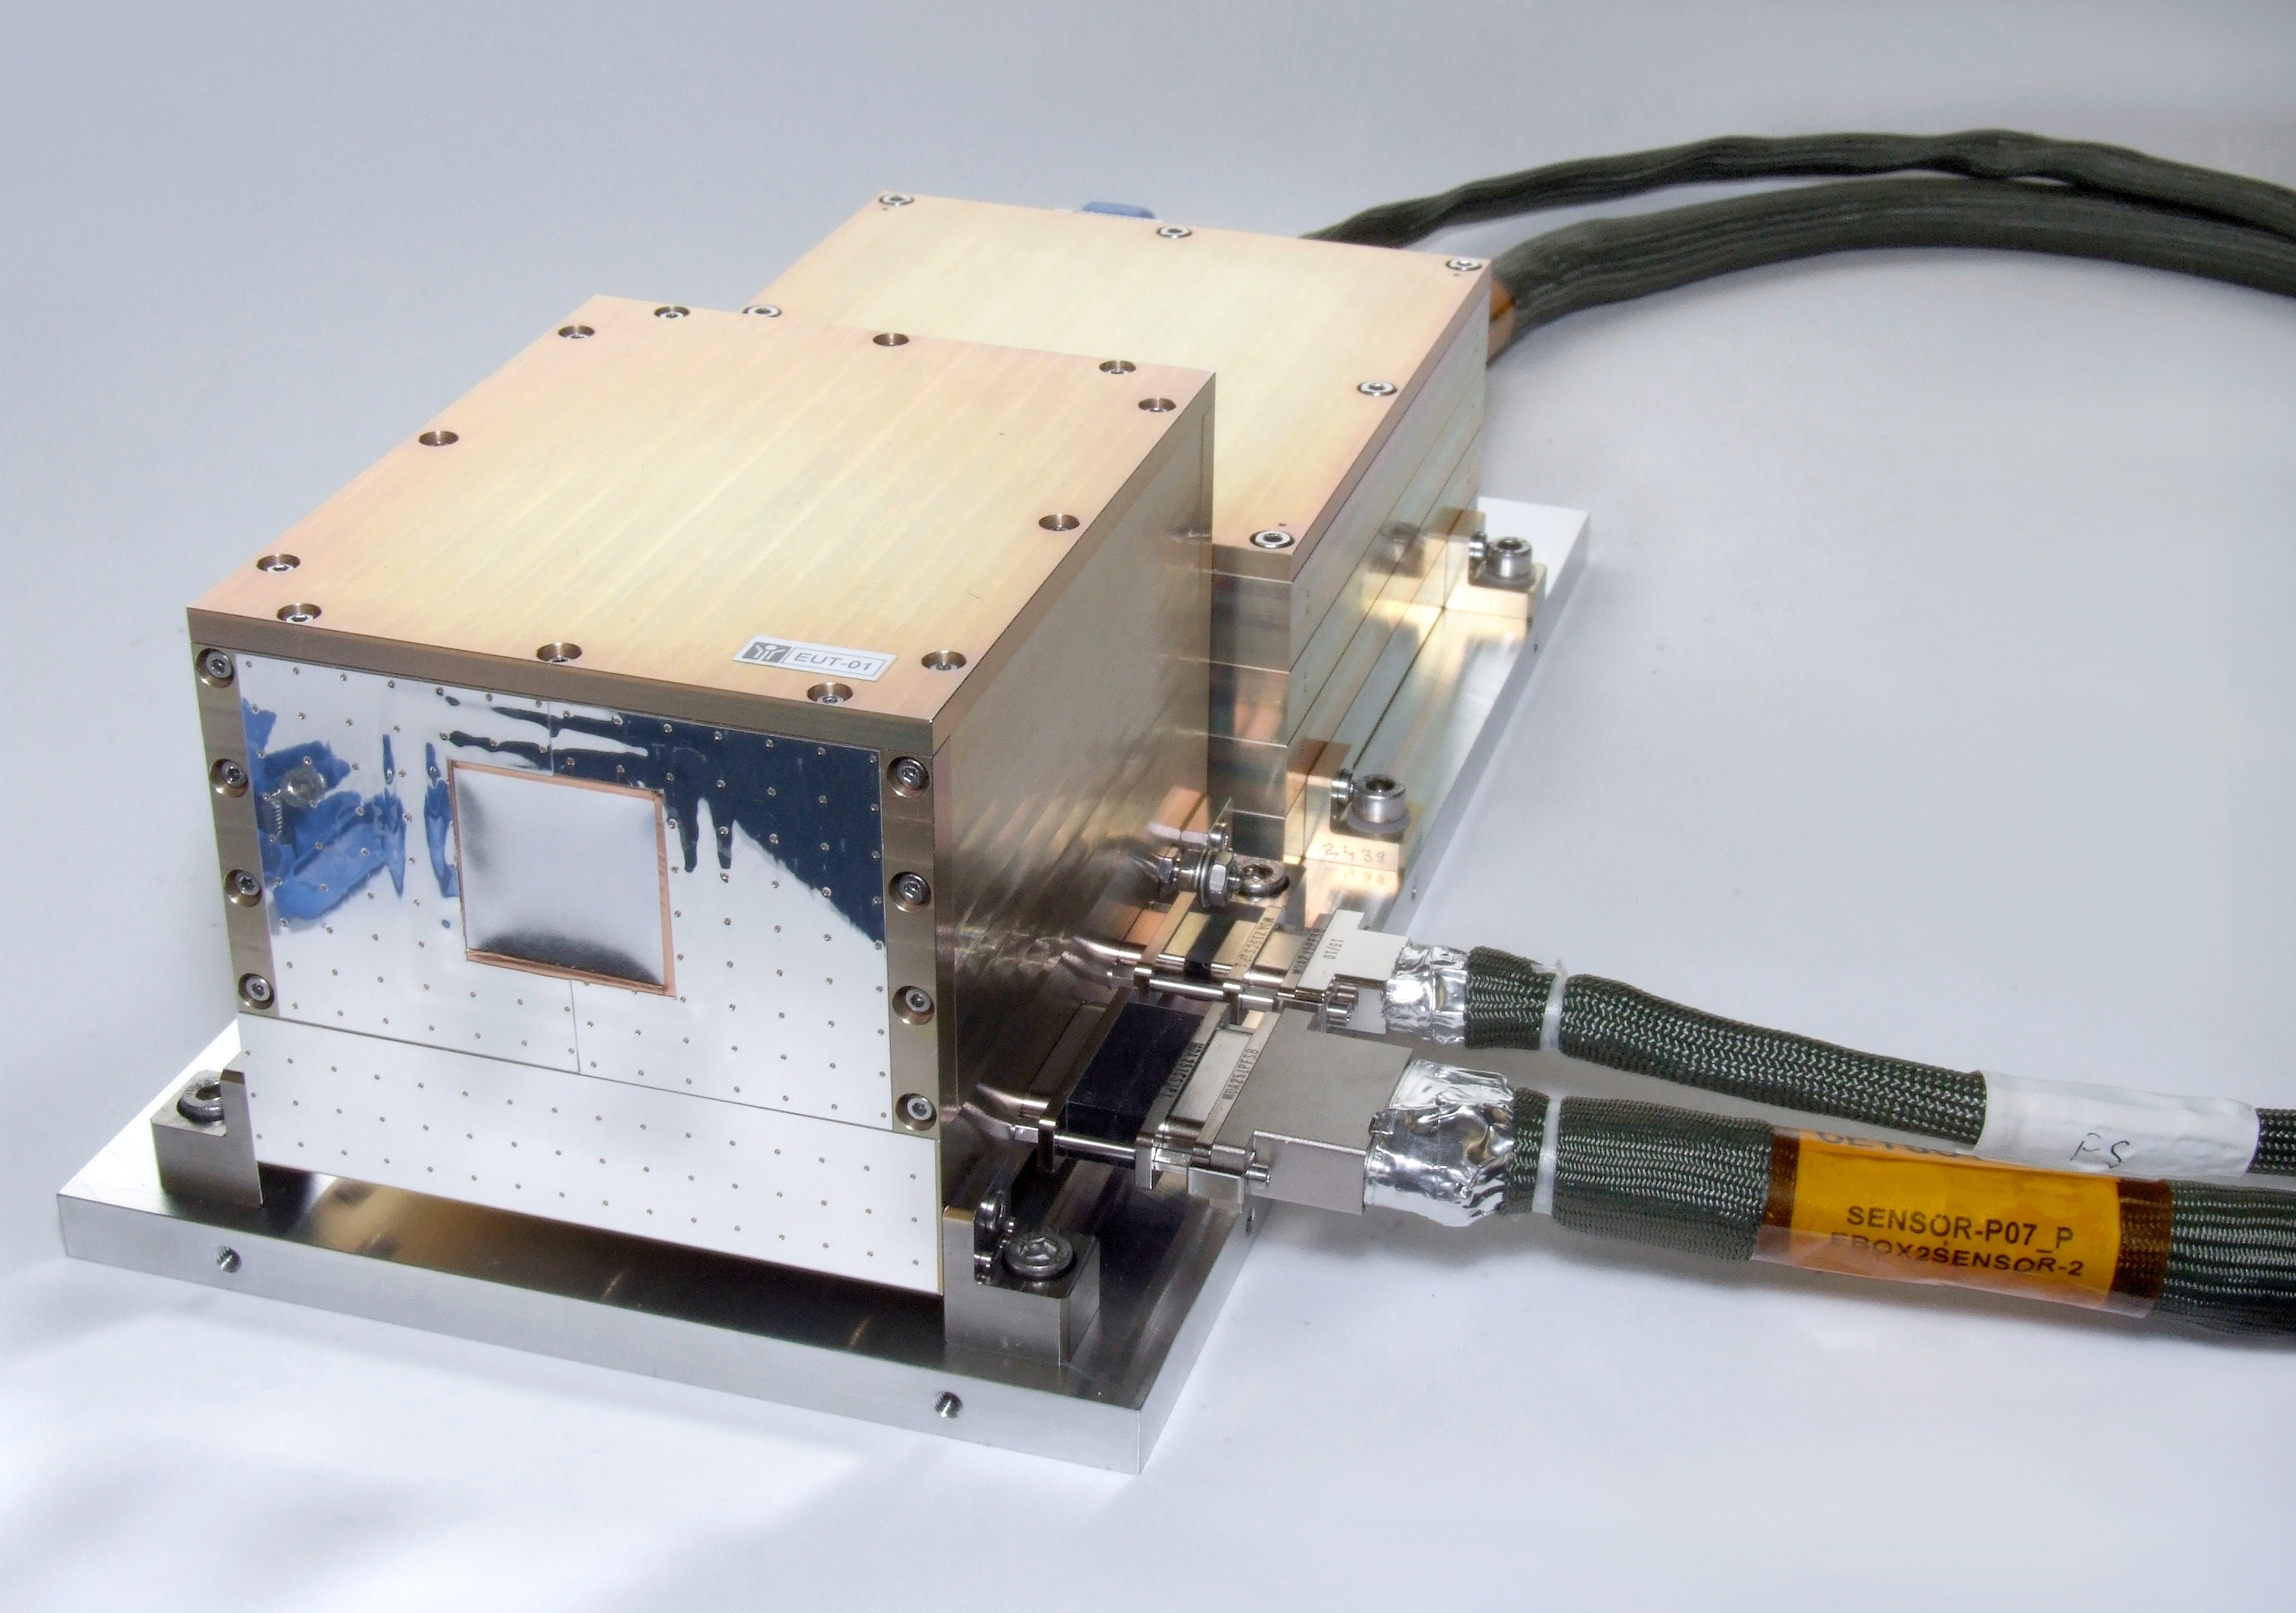
\includegraphics[width = 0.9\textwidth]{images/LND_2018-11-13.JPG}
    \caption[Photograph of Lunar Lander neutron dosimetry experiment]{The photographs of LND instrument, including the sensor head (SH, front), and electronics box (EB, rear), and 1-meters data and powver harness that connects the SH and EB. The figure was from \citet{Wimmer-2020-LND} which is actually the flight spare model of LND and was token on 2018-11-23 for the instrument paper}
    \label{Fig:LND_instrument}
\end{figure}

\begin{figure}
    \centering
    \includegraphics[width = 0.8\textwidth]{images/change4_lnd-c9_trigger-cones-colored.pdf}
    \caption[The inner structure of LND sensor head]{The skeptical view of the inner structure of the sensor head. Ten 500 $\mu$m Si \acp{SSD} are assembled in order. The different color regions indicate the \ac{FOV} of different measurement combinations. The figure was from \citet{Wimmer-2020-LND} and more detailes could be found in instrument paper.}
    \label{Fig:LND_sensor_head}
\end{figure}
Chang'E-4 is a robotic spacecraft mission of China exploring the lunar far-side surface, which is also the first human soft-landing missions on the lunar far-side surface \citep{Li2021SSRv}. The whole mission consists of a lander, a rover named Yutu-2 and a relay sattellite named Queqiao which works in the lunar orbit and connects the lunar far-side surface and the ground. The mission was launched on December 8, 2018 and successfully landed on the Von K\`arm\`an crater near the south pole of Moon on January 3, 2019 \citep{Wu2019NatGe}. Due to the extreme temperature variations on the lunar surface, the rover, lander, and scientific payloads onboard go into hibernation during the approximately two-week-long lunar night to conserve power and protect the detectors.  After a long 'sleep' night, the instruments onboard are awakened by sunlight and start measuring during the daytime. The design life time of the mission is at least one year. Obviously this target have been surpassed and so are the scientific instruments.

As one of the international scientic payload onboard Chang'E-4 mission, \ac{LND}\acused{LND} is designed by the Kiel University from Germany, with the coorperation with NSSC. The initial designed purpose of \ac{LND} is to measure the first active radiation dose rate and monitor the radiation environment caused by the changed and neutral (neutrons and $\gamma$-ray) particles, in preparation of the future human exploration of the Moon and solar system.
The main scientific objects of LND, as indicated in the instrument paper \citep{Wimmer-2020-LND}, are the following:
\begin{itemize}
    \item Dosimetry for human exploration of the Moon: LND is designed  to determine the temperal variations of the dose rate and the LET spectra which will be used to derived the quality factor \textit{Q} which is an key factor to interprete the dosimetric data.
    \item Contribution to the heliospheric science: The particle fluxes and time series of the flux are measured on the far-side of the Moon. Due to its additional measurement location, those new data can be of great help in understanding the propagation of the particles.
\end{itemize}
\ac{LND} also has two technological demonstration objects which are \textit{Determine the subsurface water content in the South-Pole Aitken Basin} and \textit{Determine the FeO content in the South-Pole Aitken Basin}.\citep{Wimmer-2020-LND}

To achieve the above scientific objects, LND measures and provides the data products including up to 1-minute charged and neutral particle dose rate measured in Si, up to 1-minute cadence LET spectra, 1-minute neutral particle deposition energy spectra, 10-minutes count rates of thermal neutrons and high time resolution (1-minutes, 10-minutes) charged particles flux and high energy resolution spectra including electrons and ions from proton to iron.

Up to May 2023, LND has been working on the lunar far-side surface for more than 4 years ($\sim$ 50 Lunar days, since 2019.1.3), have largely surpassed its designed life time.
One of the easiest way to check whether LND is working or not is looking up during night and checking whether you can see a new moon or the moon in the last/first quarter phase, which indicates that moon is moving out of the earth's shadow and the far-side of moon is facing the sun.

According to the the operations and experiment schedule from the ground, \ac{LND} has been completely or partly (more than half lunar day) switched off on the 6th, 44th, 45th lunar days. Up to May 2023, when the thesis finished, we have received the 46 lunar days data from January 2019 to the end of November 2022 which are stored in the server of Kiel group. The data have officially been publishing in the Lunar and Planetary Data release system \footnote{\url{moon.bao.ac.cn}}, where you could find the data until December 2022. 
The alternative downloading options include NASA Space Science Data Coordinated Archive and, ESA's archive ESDC (ESAC Science Data Center) which are still in building. We hope the instrument can keep running in the farside and we can receive more interesting data in the future with the increasing solar activities.


It is worth noting that we have implemented several configuration changes after \ac{LND} delivered and launched. Every morning of lunar day, 14 extra commands are uploaded to control unit of LND, in order to fix software issues and malfunction issue. The software issues are due to mistakes in the software pipeline which use the wrong channels to determine the particle energy and mistakes in the simulation when design the data products. The later affects the position of \ac{dps} boxes in the X-mas plot (See below and \citet{Wimmer-2020-LND} for more details). Neverthless, the impact on the data products is minor. 
Desipite this, the major changes of the data products are caused by raising the threshold of noise channels and removing A2 channel (the outer segement of front A detector, see Appendix in Section ** for more details of this change) in the level 3 trigger logical. The reason that we need to implement such changes are due to the skyrocket of the noise level in detector A, G, H I and J. On the 3rd and 4th lunar day, \ac{LND} was switched off for a short periods but left the lid open, which should be close to keep the sensor warm. Though the temperature on the lunar surface is increasing as sun rising, \ac{LND} and its detectors are keeping lose heat after switching off and the temperature droped dramastically in the sensor head. Such a temperature variation caused an unrecoverable deformation to the carrier and its attached detectors, especially the one in the front side and bottom side, i.e. det A and I/J. In the end the lower energy noise ($\sim$ 10 - 200 keV) largely increase.

By implemmenting the above mentioned changes, we have sucessfully reduced the noise level and mitigated its impact on the final data products. However, the damage to other data products is significant. For instance, we partly lose the measurement of minimum ioninzing particle after the increment of the threshold of I detector, and the geometry factors of two \ac{LET} spectra and penetrating particle are reduced dramatically after we disable A2, a channel playing a key role in \ac{LND}'s measurement logic. The details of the configuration changes are given in the Appendix of chapter \ref{} and the corresponding changes of the original code in the LND data processing software is given in the appendix [if you have time to do it]



\subsection{LND as a Charged particle telescope}

Due to the special design of the sensor head, \ac{LND} could be used as a dosimeter, neutral telescope and charged particle telescope. Since we mainly used the charged particle measurement in the following chapter, we will put our focus on the charged particle telescope in this section and a brief introduction of the other two are given in the next section.

The flight spare model of \ac{LND} which is a copy of the flight model running on the moon is photographed and showed in Fig.\ref{Fig:LND_instrument}. There are two seperate parts, the sensor head (SH) in the front and the electroninc box (EB) at the rear, which are connected by a 1-meter cable to provide power and transfer data. 
The SH consists of 10 Si \acs{SSD} of norminal 500 $\mu$m thickness. They are labeled from A to J and assembled in a charged-particle telescope configuration as Fig.~\ref{Fig:}.

The structure of the telescope can be divied into two parts. The upper half consists of four detectors (A, B, C, D) with A placed away from the others. A detector is the most important one in \ac{LND} sensor head, since all the charged-particle data products only count particles that have triggered the front detector A. B/C/D are assembled closely in the space in order to perform an anti-coincidence measuremet in the inner C segements. Such a detector arrangement is similar to the Flight Radiation Environment Detector (FRED) \citep{moeller-etal-2013, moeller-etal-2013b}. The lower half consists three detector pairs (E/F, G/H, I/J) which are closely packed together and an Al-Gd-Al absorber which is for the thermal neutrons. A 20 $\mu$m thickness Gd foils is insert into E/F and G/H and sandwiched structures are formed to detect the thermal neutrons. This charged particle telescope is completed by the last detector pair I/J.

By measuring the energy depostion in different \acp{SSD} and using the dE/dX - E or dE/dX - dE/dX method, depending the energy of primary particle, LND can easily identify the particles energy and species. 
The averaged energy loss of the charged particle along their travel path depends on the nuclear charge $Z_1$ and the incident velocity $\nu$. 
Such relationship could be expressed by the well-known Bethe-Bloch formula \citep{bethe-1930, bloch-1933}:

\begin{equation}
    \frac{\dd E}{\dd x} = - \frac{Z_1^2 e^4 n_e}{4 \pi \cdot \varepsilon_0^2 \beta^2 c^2 m_e} \cdot \left[ \ln\left(\frac{2 m_e  \beta^2 c^2}{\braket{E_B}}\right) - \ln(1 - \beta^2) - \beta^2  \right], 
    \label{eq:BB}
  \end{equation}
where $c$ is the speed of light, $\beta = \nu/c$, $E_B$ is the ionization energy of the medium that particle pass, and $n_e$ is the electron density in the medium, $m_e$ is the electron mass, and constant $varepsilon_0$ is the permittivity of free space.



In the energy range that \ac{LND} covered, since the $ln(\beta^2)$ hardly change, the above function could be simplified as:
\begin{equation}
    E_A \propto \frac{Z_1^2 m_1}{E_{\mathrm tot}},
    \label{eq:BB2}
\end{equation}
The products of $E_A$ and $E_{tot}$ is proportional to the nuclear charge and the mass of elements which only depend on the particle species. Hence, the composition of particles are determined. Notely, \ac{LND} could discriminate the the isotopes of elements, for instance Helium-3 and Helium-4, with limited resolution and precison in the Xmas plot (Fig.~\ref{Fig:measurement_Xmas}). However, the telescope like \ac{LND} have   Note that the nuclear charge $Z_1$ is equal to the number of protons in the nucleus, i.e. the atomic number $Z$ of the elements. When traversing the front foil of \ac{LND} sensor head, the partially charged particle like \ac{ACR} which are singly charged \citet{}, will be ionized and stripped the electrons, becoming fully charged \citet{Swaczyna2017ApJ}. Therefore,

The charged particles that LND measurement can be divided into two categories: stopping particles with energy between $\sim$ 8 MeV/nuc and $\sim$ 35 MeV/nuc and penetrating particles with energy above that range.

In Fig.~\ref{Fig:LND-Boehm-plot}, a plot generated by the large counting statistic \ac{Geant4} simulation illustrates how the stopping particles are seperated by using the $E_{tot} * E_A$ as the y-axis and $E_{tot} / E_A$ as the x-axis. The data points represents particles that stop in the detectors (B-I) with the energy up to $\sim$ 35 MeV/nuc and are simulated in \ac{Geant4} based on a carefully construced \ac{LND} instrument model. This model include all the structures inside of the sensor head, including PCB next to the detector stacks and the outer shell of sensor head. However, since we do not have the structure information of the Chang\'E-4 lander, a comprehensive model including the surrounding materital of LND is impossible. 
A screenshot of the LND model is given in the appendix [Find one and add]

Above that energy are the penetrating particles which, as the name indidcated, can penetrate detector A to I and stop in J or even penetrate J with more energy. The majority of the penetrating particles are fully penetrating particles, which means we can not measure the total energy directly. The \acp{MIP} are one of the fully penetrating particles that have extremely large initial energy from hundreds MeV to GeV but only deposit minimum energy in the detector stacks.
Since we can not measure the total energy of particle, a similar plot like Fig.~\ref{Fig:LND-Boehm-plot} for penetrating particles is not possible. Instead, we change the formula of x-axis and y-axis to $E_I/E_A$ and $dE$ respectively. The $E_I$ is the energy deposit in the last detector I. The $dE$ is the summed energy deposit in the B, C, and D.

Noteablely, the directionnal information of the particle incident from above or beneath could be possible obtained from the penetrating data. For the particle incident from above, typically $E_I/E_A$ is larger than 1 and vice veras for the beneath incident particle. 
Based on this information, we can identify the albedo protons from different branch in the 2-D histogram which is part of the Xmas plots.
The details of the derivations of albedo protons are given in Section. ~\ref{}

All the data products can be derived from the Xmas Plots of LND.

\begin{figure}
    \centering
    \includegraphics[width=0.8\textwidth]{images/LND_Boehm_plot_isotropic_on_top_of_A_annotated.png}
    \caption[LND Boehm plot of stopping particles based on the simulated data]{The different particle species are well discriminated in this LND Boehm plot which is a scatter plot of the \ac{LND} simulation data generated by the \ac{Geant4} tools \citet{Agostinelli-2003}. An isotropic source is placed on the top of A detector when the simulation is running.}
    \label{Fig:LND-Boehm-plot}
\end{figure}


\subsection{LND as dosimeter and neutral telescope}

\ac{LND} measure the \ac{TID} based the energy deposition and corresponding energy spectrum in the B inner segement. The C inner segement, which is surrouded by the B, D and C outer detector and in anti-coincidence with
all other detector segments, is used to measure the neutral dose rate including both fast neutron and $\gamma$-rays radiation. The above two are the primary data products and have good quality. 

The thermal neutrons are measured by E/F, G/H pairs which clamp a Gd-foil. The Gd-foil has a large cross section for the thermal nentron and can easily react to those neutrons. In the calibration experiment, \ac{LND} can clearly observe the neutrons by comparing the discrepancy of energy spectrum between E (G) and F (H) for neutrons coming from front (back) \citet{Wimmer2020SSRv}.
However, in real measurements, the quality of thermal neutron data is unexpectedly low due to various factors. Among these factors, the most significant one is the neutron background emitted from the \ac{RTG} and \ac{RHU}. These radioactive sources generate heat to protect the lander and payload from the frozen night, but on the other hand, leading to increased neutron background interference. The preciously measurement of those radiaion sources were unavaiable, and only an experimental estimation of these effect on the data were made by \citep{Hou2020-LNDbackground}, based on the laboratory test on the Earth and mento-carlo simulations. The results  confirmed the non-negligible background interference and provides the first attempt to remove the background from dose rate measurement. The other factors are the noise on those detectors. Like the noise channels we mentioned before, channels F2, G2 and H1 have also been troubled by the increased noise level. The L1 counters saw the count rate increased from $10^3$ count/min to $10^6$ count/min. Besides, such increase caused a significant dead time issue on the neutron dose since the neutron measurements share the same buffer. Therefore, the corresponding threshold of noise detector need to be raised to hundreds keV, as a result, we lost the data from the thermal neutrons.

The remain data products related to the radiation are \ac{LET} spectrum. \ac{LND} provide three type of \ac{LET} spectra including \ac{LET} $ABC\bar{I}$, $\bar{A}BIJ$ and $ABIJ$. Those \ac{LET} spectra can be used to derived the quality factor (Q) which then multiple the absorbed dose rate and lead to the dose equivalent. [,conference citation]
In the appendix of Chapter [], we provide the change of geometry factor of the LET spectra after implementing the configuration changes.
More details of the data products can be found in the instrument paper \citet{Wimmer2020SSRv}.

The first scientific result of \ac{LND} regarding the radiation environment on the lunar surface are reported in \citep{Zhang-2020-LND-firstresults}. In this paper, the \ac{TID}, neutron dose and \ac{LET} spectra of the first two lunar day were analyzed and presented. This is first ever dynamic measurement of the radiation variation on the lunar surface. According the measurement, the averaged total absorbed dose rate in silicon is about 13.59$\pm$1.01 $\mu$Gy/hour and among that the neutral particles account for $3.10 \pm 0.43 \mu$Gy/hour. 



\subsection{Primary data products: Xmas plots}
\begin{figure}
    \centerfloat
    \includegraphics[width =\textheight, height = 0.6\textheight, angle = 90]{images/xmas-2019-01-03To2022-11-29.png}
    \caption[LND Xmas plot based on the measurement between 2019.1.3 and 2022.11.29]{The complete Xmas plot (274 $\times$ 64) of LND based on the measurement between 2019.1.3 and 2022.11.29. All the data products could be found in this plot, including neutrals, \ac{LET} spectra, \ac{TID}, stopping and penetrating charged particles, including electron, protoon, helium and heavy ions. The corresponding simulation version could be found in \citep{Wimmer2020SSRv}}
    \label{Fig:measurement_Xmas}
\end{figure}
\clearpage
Fig.~\ref{Fig: measurement_Xmas} is the so-called "Xmas plot" \footnote{It was the front cover of the Xmas card of IEAP group in 2017, hence got the name.} of the LND. 

Xmas plot actually is an image of \ac{LND}'s memory space shaped in a 274 $\times$ 64 matrix. LND is the principal data products and all others are extracted from it every hours. Each pixel in the Xmas plot servers as a counter. After LND obtaining the deposited energy in each detector for an effective signal, the L3 trigger will calculate onboard the right position of this signal in the Xmas plot and increment the corresponding counter. 

Unlike the simulated version in \citep{Wimmer2020SSRv}, here we displayed the real measurement data from 2019.1.3 to 2022.11.29, sum up of all the data we accumulated since the first lunar day. The green rows are the memory space will not be transmitted to the ground, to save the telemetry bandwidth. The major different compared with the Xmas plot in \citep{Wimmer2020SSRv} is that LND measure not only the particle incident from above but also the albedo particles moving upward, while in the simulation, we did add the albedo component. It is obvious that in the penetrating panel of Xmas plot,  a higher than backgrond branch strech from middle to the left side. This branch represents the protons moving upward with enough energy fully penetrating all the detectors as well as the extra shielding from the lander structure. More details of how to derive albedo proton flux are given in Section.~\ref{sec:albedo_proton}.
The detailed explanations of the format of the Xmas plot are given in the \citep{Wimmer2020SSRv}


\section{Solar orbiter and High energy telescope}

Successfully launched on Feb 10, 2020, \ac{SolO} missions \citet{Mueller-2020-SolO} is an international mission cooperated between \ac{ESA} and \ac{NASA} with the aim to understand the sun and how it control the so-called helisphere. As indicated in the mission paper, the following scientific questions will be answered and further studied: (a). What drives the solar wind and where dose the coronal magnetic field originate from? (b). How do solar transients drive heliospheric variability? (c). How do solar eruptions produce energetic particles radiation that fills the heliosphere? (d). How does the solar dynamo work and drive connections between the Sun and the heliosphere?

%After finishing the cuise phase which started at June 14, 2020, \ac{SolO} has been operating in the nominla mission phase since Nov 26, 2021 as scheduled.

The \ac{SolO} has a special designed elliptic helioscentric orbit with the closest perihelion of 0.29 AU (about 42$\times10^6$ km). Using several gravity assistance during the venus flyby and earth flyby, the orbit of \ac{SolO} will gradually tilt away from the ecliptic plane and in the end can be 24 degrees above the Sun's equator. Up to May 2023 \ac{SolO} is still following an elliptical orbit circling the sun, with a maximum solar latitude of 8.66 degrees. \ac{SolO} has finished 5 perihelions with closest distance of 0.292 AU on Sep 3, 2022, and has started its 6th orbit, moving away the Sun. 
%Three time Venus flyby happened on Dec 27, 2020,  Aug 9, 2021 and Sep 4, 2022. The Earth GAM happend on Now 27, 2021.
%The above mentioned solo tragjectory information is taken from the Solar orbiter Consolidated Report on Mission analysis \footnotes{\url{https://issues.cosmos.esa.int/solarorbiterwiki/display/SOSP/Trajectory+Overview+-+10+February+2020+Launch}}

Benefit from the special position of \ac{SolO} during this trip, the multiple scientific instruments onboard the \ac{SolO} could further advanced our understanding of the sun and its affects on the heliosphere.
%in the relative field for instance the questions regarding solar coronal, solar magnetic field, solar wind, \ac{SEP}.
\ac{EPD} \citet{RodriguezPacheco-2019-EPD} is one of such scientific payload suite onboard \ac{SolO}, measuring the energetic particles over a large scale from few kev to GeV, including different plasma population of lower energy solar wind,  $\sim$ keV suprathermal particle, high energy \acp{SEP}, \acp{ACR} and \ac{GCR}. The spectra, composition, time variations and directional distributions could be obtained and derived.
\ac{EPD} comprises four different sensors, \ac{SIS}, \ac{STEP}, \ac{EPT} and \ac{HET}. 
\ac{SIS} is a time-of-flight mass spectrometer that measures ion composition from $\sim$ 0.1 - few MeV nucleon$^{-1}$. \ac{STEP} measures electrons and ions with lower energies between 4 keV and 80 keV. The special design of \ac{STEP} allows it to have high pitch-angle resolution.
\ac{EPT} and \ac{HET} share the same electronics and two identical sensor units are perpendicularly assembled on \ac{SolO}, thus detecting the particle incident from four directions. \ac{EPT} measures medium energy electrons and ions between 25 keV and 400 keV ($\sim$ 6 MeV for protons), while \ac{HET} completes the higher end, measuring electrons from 300 keV to 30 MeV and ions from 6.8 Mev/nuc to $\sim$ 100 MeV/nuc in the nominal data products. Particularly, the penetrating data products could extend the energy coverage of \ac{HET} up to $\sim$ GeV/nuc. \citet{Elftmann-2020-PhD}
The complete energy coverage of those four instruments for different particle species are given in Fig.~\ref{Fig:EPD-energy-coverage}.
In the following section, we briefly introduce the details of \ac{HET}, which is mainly used in this study. Further details of the other three parts can be found in the instrument paper \citet{RodriguezPacheco-2019-EPD} and the first years overview paper from \citep{Wimmer2021AA}.


\begin{figure}
    \centering
    \includegraphics[width = \textwidth]{images/EPD_coverage.png}
    \caption[The energy coverage of EPD instruments]{The energy coverage of different \ac{EPD} instruments for different partidcle species. This figure is an updated version of energy coverage plot made by \citep{JohanPhd2020}, based on the similar plot from \citep{RodriguezPacheco-2019-EPD}. We reproduced it here. In this figure, the HET measurements are splited into stopping and penetrating parts. The later one can largely extend the measurement ability of HET \citet{Elftmann-2020-PhD}.}
    \label{Fig:EPD-energy-coverage}
\end{figure}  

\subsection{High energy telescope}

\begin{figure}
    \centering
    \includegraphics[width = \textwidth]{images/het.png}
    \caption[The HET sensor head]{The cross profile of HET sensor head. The detector names are labeled. (Figure reproduced from \citep{RodriguezPacheco-2019-EPD})}
    \label{fig:HET-sensor-head}
\end{figure}

\ac{HET} is a double-ended telescope. In FIg.~\ref{fig:HET-sensor-head}, we give the cross profile of the \ac{HET} sensor head. The sensor head of \ac{HET} consists of four 300 $\mu$m silicon \ac{SSD} stacks, with two in each side (A1, B1 in the front side and A2, B2 in the back side), and a 2-cm thickness bismuth germanium oxide ($Bi_{4}Ge_{3}O_{12}$ , BGO) scintillator (detector C) in the center. Suchs setup is similar to \ac{RAD} which is another instrument developed by Kiel Univeristy and is running on the Mars surface.  

HET use the $\mathrm{dE/dX - E}$ technique to discriminates different particle species of different energy, including electron, proton, helium-4, and heavy ions like carbon, nitrogen, oxygen, and iron. This method is the same as the measurement principle of \ac{LND}.

Noteablely, in order obtain the pitch-angle distribution of high energy particle in the magnetic field, especially during the onset phase of \ac{SEP}, two HET units, HET1 and HET2, are equiped on the \ac{SolO}. They are specially mounted on two perpendicular direcitons, sunward/antisunward (ecliptic) and south/north (polar). The evolution of pitch angle distribution of \ac{SEP} is of great importance in understanding the transportation process of particle in the space align with \ac{IMF} [citaion, find precious words]. 


Charged particle after they incident and penetrate the A detector (A1 or A2), can be splited into the stopping particle and penetrating particle, depending on their energy and whether they stop in detector B/C. The corresponding nominal data products, as given in Table 22 of \citep{RodriguezPacheco-2019-EPD}, are ABnC (stopping in B, 6.5 - 9.5 Me\/nuc), ABC (stoppin in C, $\sim$10 - $\sim$ 100 MeV\/nuc) and penetrating (above 100 MeV/nuc to infinity). These particle are fully analyzed by the $\mathrm dE/dX - E$ method. For the stopping particle, the primary energy and the particle direction information are directly obtained. While for the penetrating particle, the primary energy can be estimated based on their energy loss on the detector and the \ac{Geant4} simulation. The abovementioned nominal data products of HET contribute to the study of \ac{SEP}, \ac{ACR} and \ac{GCR}.


In addition to the nominal data products, it is crucial to underscore the contribution of housekeeping data in the studies.
The housekeeping data are EPD sensor produced instrumental data which have the highest priority for downlink to the Earth and are used 
it is worthnoting that the housekeeping data of HET also provide the possibility to study the \ac{SEP} events.

The nominal scientific data products of HET are designed to study SEP events of higher intensity by limiting the FOV and using coincidence measurements to discriminate species and achieve better energy resolution. However such data products are not optimal for the analysis that requires both time resolution and larger counting statistc, for instance to determine the SEP events period. Alternatively, single detector count rates without any coincidence conditions which is one of the housekeeping data, could provide the possibility to achieve better counting statistic. Von forstner et al 2021 use the single C counter to study the temporal varitation of the forbush decrease and Allen et al 2021 confirmed the drop out of C counter rate during the first venus flyby is due to the VENUS blockage on the HET FOV.

Similar with the single detector count rate, in the study, we introduce \textit{any(a1, b1)} which is a level-2 trigger of HET to determine the SEP period. \textit{a1} and \textit{b1} represent the front two SSDs of HET sensor head. This level-2 trigger counts all the particles that have energy above the threshold of detector A or detector B, which is 50 keV in the nominal mode [citaion effman thesis]. Since no obstacles in front of A detector, both electron and protons with small energys could be counted in this trigger and not a single SEP event will be missed in the change of time series of \textit{any(a1,b1)}, even though sometimes no corresponding helium-4 change reflected in the flux higher energy channels.

For more details of the inner structure and parameter of the HET, and the most update status of HET, one could refer to \citep{2020AA_EPD} and \citep{wimmer2021AA}.

% Built in a cooperation between the University of Kiel and Southwest Research Institute, the \acl{RAD}\acused{RAD} \citep[\acs{RAD},][]{Hassler-2012-MSLRAD} instrument onboard the \acl{MSL}\acused{MSL} \citep[\acs{MSL},][]{Grotzinger-2012} mission provided the first-ever direct radiation measurements on the surface of Mars. It is designed to measure both charged and neutral particles, and calculate particle spectra as well as dosimetric quantities, such as the \ac{TID} rate and \ac{LET} spectra. This aligns with its main science objectives, which include the characterization of energetic particle spectra on the surface of Mars (\acp{GCR} and \acp{SEP}) and the determination of the radiation hazard for past or present life on Mars or for future human Mars missions. Consequently, \ac{RAD} has not only been continuously measuring the radiation environment on the Martian surface since the \textit{Curiosity} rover's landing on August 6, 2012, but has also been active during the most part of its 9-month flight to Mars (the so-called cruise phase) to evaluate the radiation dose that astronauts would be exposed to when traveling to Mars.



% \begin{figure}
% 	\centering
% 	\includegraphics[width=0.4\linewidth]{images/rad}
% 	\caption[Photo of the \acs{RAD} sensor head]{A photo of the \ac{RAD} sensor head before it was mounted on the \ac{MSL} spacecraft. The red protection cap was removed after installation on the rover. Source: NASA/JPL-Caltech/SwRI}
% 	\label{fig:rad-photo}
% \end{figure}

% The \ac{RAD} sensor head (shown in \autoref{fig:rad-photo}) is mounted on the top deck of the rover, pointing along the z axis of RAD, i.e. towards the zenith. It is composed of three hexagonal silicon solid-state detectors (A, B, and C) with a thickness of \SI{300}{\micro\meter} each, mounted in a stack to form a charged particle telescope (\autoref{fig:rad-sensorhead}) with an opening angle of about \SI{60}{\degree}. Each detector is divided into an inner and an outer segment.
% The D detector, a cesium iodide (CsI) scintillator in the shape of a truncated hexagonal pyramid, is situated directly below the charged particle telescope. Its shape is designed to align with the inner segment of C and follows the opening angle of the charged particle telescope (shown with dashed lines in \autoref{fig:rad-sensorhead}). The E detector, a plastic scintillator which is located below D, is mainly responsible for neutral particle detection. D and E are surrounded by another plastic scintillator (F), which is used as an anticoincidence shield to reject ions that enter D or E from the sides.

% \begin{figure}
% 	\centering
% 	%\documentclass{standalone}
%\usepackage{tikz}
%\usepackage{amsmath}

%\usetikzlibrary{calc}
%\usetikzlibrary{decorations.pathmorphing}

%\definecolor{light-gray}{gray}{0.9}

%\begin{document}
\begin{tikzpicture}[scale=0.8]
    \tikzset{%
        add/.style args={#1 and #2}{
            to path={%
                ($(\tikztostart)!-#1!(\tikztotarget)$)--($(\tikztotarget)!-#2!(\tikztostart)$)%
                \tikztonodes},add/.default={.2 and .2}}
    }  
    
    \def\bottomwidth{3.25}
    \def\midwidth{1.8}
    \def\topwidth{1.65}
    \def\bottomheight{2.5}
    \def\midheight{4.375}
    \def\Fthickness{1}
    \def\Sithickness{0.1}
    \def\BCdistance{0.15}
    \def\topheight{8.375}
    
    % FOV
    \draw[add=0 and 0.3, dashed] (\midwidth - \Fthickness, \midheight) to (-\topwidth, \topheight);
    \draw[add=0 and 0.3, dashed] (-\midwidth + \Fthickness, \midheight) to (\topwidth, \topheight);
    
    \draw[|<->|] (-\topwidth, \topheight) ++ (90+30:0.5) arc (90+30:90-30:{\topheight-\midheight-0.2}) node[pos=0.4, above] {\small\SI{60}{\degree}};

    % A
    \draw[fill=light-gray] (-\topwidth, \topheight - \Sithickness) rectangle (\topwidth, \topheight);
    \draw (-\midwidth + \Fthickness, \topheight - \Sithickness) --  (-\midwidth + \Fthickness, \topheight);
    \draw (-\midwidth + \Fthickness, \topheight - \Sithickness) --  (-\midwidth + \Fthickness, \topheight);
    \draw (\midwidth - \Fthickness, \topheight - \Sithickness) --  (\midwidth - \Fthickness, \topheight);
    \draw (\midwidth - \Fthickness, \topheight - \Sithickness) --  (\midwidth - \Fthickness, \topheight);
    \draw[latex-] (-\topwidth, \topheight - \Sithickness / 2) -- (-\topwidth - 0.5, \topheight - \Sithickness / 2) node[left] {A};
    
    % B
    \draw[fill=light-gray] (-\topwidth, \midheight + \BCdistance) rectangle (\topwidth, \midheight + \BCdistance + \Sithickness);
    \draw (-\midwidth + \Fthickness, \midheight + \BCdistance) --  (-\midwidth + \Fthickness, \midheight + \BCdistance + \Sithickness);
    \draw (-\midwidth + \Fthickness, \midheight + \BCdistance) --  (-\midwidth + \Fthickness, \midheight + \BCdistance + \Sithickness);
    \draw (\midwidth - \Fthickness, \midheight + \BCdistance) --  (\midwidth - \Fthickness, \midheight + \BCdistance + \Sithickness);
    \draw (\midwidth - \Fthickness, \midheight + \BCdistance) --  (\midwidth - \Fthickness, \midheight + \BCdistance + \Sithickness);
    \draw[latex-] (-\topwidth, \midheight + \BCdistance + \Sithickness / 2) -- (-\topwidth - 0.5, \midheight + \BCdistance + \Sithickness / 2 + 0.3) node[left] {B};
    
    % C
    \draw[fill=light-gray] (-\topwidth, \midheight) rectangle (\topwidth, \midheight + \Sithickness);
    \draw (-\midwidth + \Fthickness, \midheight) --  (-\midwidth + \Fthickness, \midheight + \Sithickness);
    \draw (-\midwidth + \Fthickness, \midheight) --  (-\midwidth + \Fthickness, \midheight + \Sithickness);
    \draw (\midwidth - \Fthickness, \midheight) --  (\midwidth - \Fthickness, \midheight + \Sithickness);
    \draw (\midwidth - \Fthickness, \midheight) --  (\midwidth - \Fthickness, \midheight + \Sithickness);
    \draw[latex-] (-\topwidth, \midheight + \Sithickness / 2) -- (-\topwidth - 0.5, \midheight + \Sithickness / 2) node[left] {C};
    
    % border of ABC
    \draw (-\topwidth, \midheight) -- (-\topwidth, \topheight);
    \draw (\topwidth, \midheight) -- (\topwidth, \topheight);
    
    % D
    \draw[fill=light-gray] (\bottomwidth - \Fthickness, \bottomheight) --  (-\bottomwidth + \Fthickness, \bottomheight) -- (-\midwidth + \Fthickness, \midheight) -- (\midwidth - \Fthickness, \midheight) -- (\bottomwidth - \Fthickness, \bottomheight);   
    \node at (0, {\bottomheight + (\midheight - \bottomheight) / 2}) {D};   
    
    % E
    \draw[fill=green!50] (\bottomwidth - \Fthickness, \bottomheight) -- (\bottomwidth - \Fthickness, \Fthickness) --
    (-\bottomwidth + \Fthickness, \Fthickness) --  (-\bottomwidth + \Fthickness, \bottomheight) -- (\bottomwidth - \Fthickness, \bottomheight);  
    \node at (0, {\Fthickness + (\bottomheight - \Fthickness) * 0.4}) {E};   
    
    % F
    \draw[fill=Dandelion!50] (-\bottomwidth, 0) -- (\bottomwidth, 0) -- (\bottomwidth, \bottomheight) -- (\midwidth, \midheight) --
    (\midwidth - \Fthickness, \midheight) -- (\bottomwidth - \Fthickness, \bottomheight) -- (\bottomwidth - \Fthickness, \Fthickness) --
    (-\bottomwidth + \Fthickness, \Fthickness) --  (-\bottomwidth + \Fthickness, \bottomheight) -- (-\midwidth + \Fthickness, \midheight) --
    (-\midwidth, \midheight) -- (-\bottomwidth, \bottomheight) -- (-\bottomwidth, 0);     
    \node at (0, \Fthickness / 2) {F};
    
    % trajectories of ions
    \draw[thick, green, -latex] (-\topwidth*0.7, \topheight*1.25) node[above, align=center] {\small Ion\\ \small (accepted)}
     -- ({-(\midwidth - \Fthickness) * 0.5}, \midheight + \Sithickness / 2);
    \draw[thick, green, -latex] (\topwidth*0.65, \topheight*1.25) node[above, align=center] {\small Ion\\ \small (accepted)}
     -- ({-(\midwidth - \Fthickness) * 0.5}, {\bottomheight +  (\midheight - \bottomheight) / 2});
    \draw[thick, red, -latex] (0, \topheight*1.4) node[above, align=center] {\small Ion\\ \small (rejected)}
     -- (0, \topheight - \Sithickness / 2);
    \draw[thick, red, -latex] (\bottomwidth, \midheight) node[above right, align=center] {\small Ion\\ \small (rejected)}
    -- (\bottomwidth * 0.4, {\bottomheight + (\midheight - \bottomheight) * 0.2});
    
    % trajectory of neutron
    \draw[thick, gray, -latex] (-\bottomwidth*0.3, -0.5) node[below] {\small Neutron (accepted)}
    -- (-\bottomwidth*0.3, {\Fthickness + \bottomheight * 0.2});
    \draw[thick, gray, -latex]  (-\bottomwidth*0.3, {\Fthickness + \bottomheight * 0.2}) -- (-\bottomwidth * 1.1, \bottomheight * 1.3);
    \draw[thick, blue, -latex]  (-\bottomwidth*0.3, {\Fthickness + \bottomheight * 0.2}) -- (0, \bottomheight * 1.1) node[midway, right, xshift=1mm] {\footnotesize Recoil proton};
    
    % trajectory of gamma
    \draw[thick, gray, decorate, decoration=snake] (-\bottomwidth*1.2, \bottomheight * 0.8) node[below, align=center, xshift=-4mm] {\small $\gamma$-ray\\ \small (accepted)} -- (-\bottomwidth * 0.3, \bottomheight * 1.4);
    \draw[thick, gray, -latex] (-\bottomwidth * 0.3, \bottomheight * 1.4) -- ++ (\bottomwidth * 0.03, \bottomheight * 0.02);
    
\end{tikzpicture}
%\end{document}
% 	\caption[Schematic diagram of the \acs{RAD} sensor head]{Schematic diagram of the \ac{RAD} sensor head. Red, green, blue and gray arrows show possible trajectories of charged and neutral particles through the detectors. Based on      \textcite{Hassler-2012-MSLRAD}, Fig. 7b}
% 	\label{fig:rad-sensorhead}
% \end{figure}

% For the detection of charged particles, \ac{RAD} requires an energy deposit in at least the A and B detector, which sets the lower limit for the particle's kinetic energy to e.g. \SI{6}{\mega\electronvolt} for protons. Higher energy charged particles penetrate the B detector and stop in C, D, or E, where the high stopping power of the D detector allows for a large energy range, e.g. up to \SI{95}{\mega\electronvolt} for stopping protons. For stopping charged particles, the charge and the total kinetic energy can be determined from the two measured quantities, the total deposited energy $E$ in all triggered detectors and the \ac{LET} (deposited energy per path length) $\dd E/\dd x$ in one of the detectors. This common principle is called the $\dd E/\dd x$-$E$ method and has been in use in numerous instruments since the IMP-\liningnums{1} mission in the 1960s \citep{McDonald-1964}.

% Higher energy charged particles, which penetrate the whole \ac{RAD} sensor, cannot be analyzed using this technique, as the total energy $E$ is not measured directly in this case. Up to a few hundred \si{\mega\electronvolt} per nucleon, particles can still be partially analyzed as their \ac{LET} is slightly different at the top and bottom ends of the telescope. In this case, the \ac{LET} ratio between the top and bottom can be used to infer the approximate kinetic energy of the incoming particle. For even higher energy particles, the so-called \acp{MIP}, there is no significant change in the \ac{LET}, so only the charge and \ac{LET} can be determined, but not the primary energy.

% The D and E detectors are both, to different degrees, also sensitive to neutral particles. Being a CsI scintillator, D can detect secondary electrons produced by $\gamma$-rays effectively, while neutrons hitting E can interact with the hydrogen atoms in the plastic to produce recoil protons. An inversion method that takes all these interaction processes into account is then used to derive neutral particle spectra \citep{Koehler-2011}.

% Being an instrument with a rather low mass (\SI{1.6}{\kilogram}) and volume, the observation of short-term and low-amplitude \ac{GCR} variations such as Forbush decreases with \ac{RAD} is only possible when measuring particles that enter the sensor head from all directions, as the restricted opening angle of the charged particle telescope decreases the count rate too much. In this case, the dose rate data products of \ac{RAD} can be used, which are available for the B and E detectors. The E detector is best suited for this purpose due to its larger volume and therefore better statistics.
% The dose in a detector is calculated as
% \begin{equation}
% D = \frac{E_\text{dep}}{m},
% \end{equation}
% i.e. the total energy deposited in the detector divided by its mass, and typically given in units of $\si{\gray} = \si{\joule\per\kilogram}$. The dose rate is its time derivative, so it is given in \si{\gray\per\second} (or \si{\micro\gray\per\day}, for the order of magnitude that is typically observed on planets). In comparison to a simple count rate, where each detected particle increases the counter by one, particles stopping in the detector typically contribute more to the dose rate than penetrating particles, as the former deposit all their energy.

% Because \ac{RAD} is located on the surface of Mars, incoming primary \ac{GCR} and \ac{SEP} particles first need to travel through the Martian atmosphere before reaching the \ac{RAD} detectors. In this process, some particles are shielded away, while others can generate secondary particles by interacting with the particles in the atmosphere. Thus, the radiation environment observed by \ac{RAD} is a mix of primary and secondary particles, and \ac{RAD} measurements cannot be directly compared to deep-space detectors without taking into account the atmospheric response functions \citep[see e.g.][]{Guo-2017,Guo-2019}. For example, \ac{SEP} events need a certain minimum energy to be observed on ground, so \ac{RAD} only sees the most intense events as a \ac{GLE}.

% The atmospheric pressure measured by the \ac{REMS} instrument onboard \ac{MSL} shows a significant daily variation of about $\pm\SI{5}{\percent}$ \citep{Haberle-2014} due to the considerable temperature changes between day and night --- for comparison, the diurnal pressure variations on Earth are at least an order of magnitude lower \citep[e.g.][]{LeBlancq-2011}. These pressure variations also influence the \ac{RAD} measurements, as they affect the column mass of the atmosphere above \ac{MSL}, and thus change the amount of secondary particles generated in the atmosphere. A clear correlation between dose rate and pressure was observed by \citet{Guo-2017}. These diurnal variations show amplitudes up to $\sim\SI{2.5}{\percent}$, and this needs to be taken into account when observing short-term variations of the \ac{GCR}, which are typically on a similar order of magnitude. The easiest solution would be to average the dose rate measurements over one solar day (sol) but this would significantly increase the uncertainty for the onset time definition of events such as \acp{FD}. Instead, a spectral notch filter can be applied to the data to filter out the 1 sol frequency and harmonics. This method was described in detail by \citet{Guo-2017-maven} and is also used for most \ac{RAD} data shown within this thesis.
% These considerations about atmospheric effects of course do not apply to the cruise phase data, where \ac{RAD} was relatively lightly shielded by the surrounding \ac{MSL} spacecraft \citep{Zeitlin-2013-cruise,guo2015cruise} and no diurnal effects were observed.

% \section{The Solar Orbiter High Energy Telescope}
% \label{sec:solohet}

% The ESA \acl{SolO}\acused{SolO} spacecraft \citep[\acs{SolO},][]{Mueller-2020-SolO} was launched successfully on February 10, 2020. During its mission, it will travel as close to the Sun as \SI{0.27}{\AU} and provide valuable measurements of all kinds of solar events with its comprehensive remote sensing and in situ instrument suite. The \acl{EPD}\acused{EPD} investigation \citep[\acs{EPD},][]{RodriguezPacheco-2019-EPD} onboard \ac{SolO}, a collaboration of the University of Kiel, the University of Alcalá and the Johns Hopkins University APL, is comprised of four instruments, covering the whole energetic particle spectrum from a few \si{\kilo\electronvolt} up to several hundreds of \si{\mega\electronvolt} (\autoref{fig:epd_energy_ranges}).
% \begin{figure}
% 	\centering
% 	%\documentclass{standalone}
%\usepackage[dvipsnames]{xcolor}
%\usepackage{tikz}
%\usepackage{amsmath}
%\usepackage{siunitx}
%\usepackage{pgfplots}

%\usetikzlibrary{calc}
%\usetikzlibrary{decorations.pathmorphing}

%\definecolor{light-gray}{gray}{0.9}

%\definecolor{red}{HTML}{d62728}
%\definecolor{orange}{HTML}{ff7f0e}
%\definecolor{green}{HTML}{2ca02c}
%\definecolor{blue}{HTML}{1f77b4}
%\definecolor{purple}{HTML}{9467bd}
%\definecolor{light-gray}{gray}{0.9}

%\begin{document}
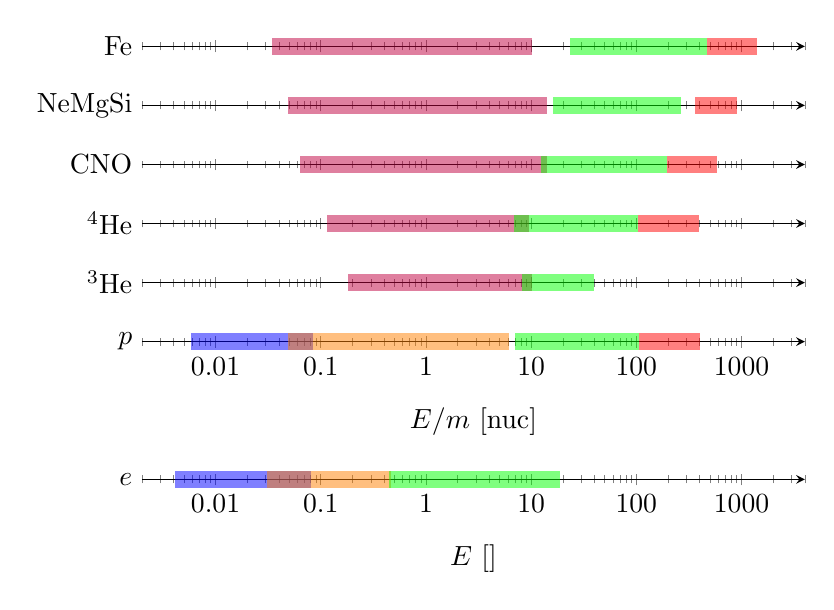
\begin{tikzpicture}
	\def\xmin{0.002}
	\def\xmax{4000}

	% EPT energy ranges, based on calibration as of 2020-10-01
	% ELECTRONS
	\begin{semilogxaxis}[xmin=\xmin, xmax=\xmax, axis x line=middle, hide y axis, ymin=-2,ymax=2,
					 height=2cm, width=10cm,
					 xlabel={$E$ [\si{\mega\electronvolt}]},
					 x label style={at={(axis description cs:0.5,-1.2)},anchor=north},clip=false,
					 log ticks with fixed point, x tick label style={/pgf/number format/1000 sep={}},yshift=0.25cm]
		\fill[blue, opacity=0.5] (axis cs:0.0041, -1) rectangle (axis cs:0.080, 1);
		\fill[orange, opacity=0.5] (axis cs:0.031, -1) rectangle (axis cs:0.47, 1);
		\fill[green, opacity=0.5] (axis cs:0.45, -1) rectangle (axis cs:18.8, 1);
		\node[left] at (axis cs:\xmin, 0) {$e$};
	\end{semilogxaxis}
	
	% PROTONS
	\begin{semilogxaxis}[xmin=\xmin, xmax=\xmax, axis x line=middle, hide y axis, ymin=-2,ymax=2,
	height=2cm, width=10cm, 
	xlabel={$E/m$ [\si{\mega\electronvolt\per nuc}]},
	x label style={at={(axis description cs:0.5,-1.2)},anchor=north},
	yshift=2cm, clip=false,
	log ticks with fixed point, x tick label style={/pgf/number format/1000 sep={}}]
		\fill[blue, opacity=0.5] (axis cs:0.0058, -1) rectangle (axis cs:0.085, 1);
		\fill[orange, opacity=0.5] (axis cs:0.049, -1) rectangle (axis cs:6.1, 1);
		\fill[green, opacity=0.5] (axis cs:7.0, -1) rectangle (axis cs:105, 1);
		\fill[red, opacity=0.5] (axis cs:105, -1) rectangle (axis cs:401.13, 1);
		%\fill[purple, opacity=0.5] (axis cs:0.24, 1) rectangle (axis cs:9.4, 3);
		\node[left] at (axis cs:\xmin, 0) {$p$};
	\end{semilogxaxis}
	
	% 3He
	\begin{semilogxaxis}[xmin=\xmin, xmax=\xmax, axis x line=middle, hide y axis, ymin=-2,ymax=2,
	height=2cm, width=10cm, xticklabels={,,},
	yshift=2.75cm, clip=false]
		\fill[purple, opacity=0.5] (axis cs:0.18, -1) rectangle (axis cs:10.2, 1);
		\fill[green, opacity=0.5] (axis cs:8.1, -1) rectangle (axis cs:39.7, 1);
		\node[left] at (axis cs:\xmin, 0) {$^3$He};
	\end{semilogxaxis}
	
	% 4He
	\begin{semilogxaxis}[xmin=\xmin, xmax=\xmax, axis x line=middle, hide y axis, ymin=-2,ymax=2,
	height=2cm, width=10cm, xticklabels={,,},
	yshift=3.5cm, clip=false]
		%\fill[orange, opacity=0.5] (axis cs:6.37, 1) rectangle (axis cs:24.51, 3);
		\fill[purple, opacity=0.5] (axis cs:0.115, -1) rectangle (axis cs:9.493, 1);
		\fill[green, opacity=0.5] (axis cs:6.877, -1) rectangle (axis cs:104, 1);
		\fill[red, opacity=0.5] (axis cs:104, -1) rectangle (axis cs:392.84, 1);
		\node[left] at (axis cs:\xmin, 0) {$^4$He};
	\end{semilogxaxis}
	
	% CNO
	\begin{semilogxaxis}[xmin=\xmin, xmax=\xmax, axis x line=middle, hide y axis, ymin=-2,ymax=2,
	height=2cm, width=10cm, xticklabels={,,},
	yshift=4.25cm, clip=false]
		\fill[purple, opacity=0.5] (axis cs:0.064, -1) rectangle (axis cs:14.13, 1);
		\fill[green, opacity=0.5] (axis cs:12.54, -1) rectangle (axis cs:197, 1);
		\fill[red, opacity=0.5] (axis cs:197, -1) rectangle (axis cs:578.37, 1);
		\node[left] at (axis cs:\xmin, 0) {CNO};
	\end{semilogxaxis}
	
	% NeMgSi
	\begin{semilogxaxis}[xmin=\xmin, xmax=\xmax, axis x line=middle, hide y axis, ymin=-2,ymax=2,
	height=2cm, width=10cm, xticklabels={,,},
	yshift=5cm, clip=false]
		\fill[purple, opacity=0.5] (axis cs:0.049, -1) rectangle (axis cs:14.13, 1);
		\fill[green, opacity=0.5] (axis cs:16.2, -1) rectangle (axis cs:268.42, 1);
		\fill[red, opacity=0.5] (axis cs:358, -1) rectangle (axis cs:915.03, 1);
		\node[left] at (axis cs:\xmin, 0) {NeMgSi};
	\end{semilogxaxis}
	
	% Fe
	\begin{semilogxaxis}[xmin=\xmin, xmax=\xmax, axis x line=middle, hide y axis, ymin=-2,ymax=2,
	height=2cm, width=10cm, xticklabels={,,},
	yshift=5.75cm, clip=false]
		\fill[purple, opacity=0.5] (axis cs:0.0346, -1) rectangle (axis cs:10.29, 1);
		\fill[green, opacity=0.5] (axis cs:23.66, -1) rectangle (axis cs:465.7, 1);
		\fill[red, opacity=0.5] (axis cs:465.8, -1) rectangle (axis cs:1388.40, 1);
		\node[left] at (axis cs:\xmin, 0) {Fe};
	\end{semilogxaxis}
\end{tikzpicture}
%\end{document}
% 	\caption[\acs{EPD} energy coverage]{Energy coverage of the different sensors in the \ac{SolO} \ac{EPD} suite for electrons and different ion species, based on the current science data products as of October 2020. This is an updated and enhanced version of Figure 3 from \citet{RodriguezPacheco-2019-EPD}. In the case of the CNO and NeMgSi groups, the responses for carbon and neon were taken as an example, the other species differ only slightly. For simplicity, \acs{SIS} protons, \acs{EPT} stopping helium as well as \acs{EPT} penetrating data products, which overlap with other measurements, are excluded from this plot. For the penetrating data products of \acs{HET}, the highest energy bin \citep[as given by][Appendix A]{Elftmann-2020-PhD} is not included, as its coverage extends to infinity.}
% 	\label{fig:epd_energy_ranges}
% \end{figure}
% The lowest energies of electrons and protons, from a few \si{\kilo\electronvolt} (slightly above the solar wind bulk) up to \SI{80}{\kilo\electronvolt}, are measured by the \ac{STEP} telescope, which is followed by the \ac{EPT} for medium energies up to $\sim\SI{6}{\mega\electronvolt}$ for protons and \SI{450}{\kilo\electronvolt} for electrons. Both \ac{EPT} and \ac{STEP} mainly measure electrons and protons, but cannot distinguish between protons and heavier ion species. Hence, they are supplemented with the \ac{SIS}, a time-of-flight based instrument that measures 12 ion species from H to Fe between \SI{14}{\kilo\electronvolt\per nuc} and \SI{20.5}{\mega\electronvolt\per nuc}. The highest energies of electrons and all ion species are covered by the \ac{HET}, whose measurements are, similarly to \ac{MSL}/\ac{RAD} (\autoref{sec:mslrad}), based on the $\dd E/\dd x$-$E$ method.

% The double-ended \ac{HET} sensor head is shown in Figure \ref{subfig:het-sensorhead-cad}. Two of these sensors are installed on the side decks of the \ac{SolO} spacecraft to provide four viewing directions: sunward, antisunward, north and south. The sunward and antisunward fields of view (\ac{HET} 1) are pointed \SI{35}{\degree} away from the radial direction within the ecliptic, which corresponds to the nominal Parker spiral direction, while the north and south fields of view (\ac{HET} 2) are pointed out of the ecliptic. The \ac{HET} telescopes each consist of four silicon solid-state detectors (A1, B1, B2, A2) and a bismuth germanium oxide (Bi$_4$Ge$_3$O$_{12}$, BGO) scintillator (C) in the center. This setup is similar to \ac{RAD}, though there is no second plastic scintillator for the detection of neutral particles.

% \begin{figure}
% 	\centering
% 	\subfloat[\acs{CAD} rendering of the \ac{HET} sensor head. Adapted from \citet{RodriguezPacheco-2019-EPD}, Fig. 31.]{
% 		\includegraphics[width=0.7\textwidth]{images/het_enhanced.png}
% 		\label{subfig:het-sensorhead-cad}
% 	}\\
% 	\subfloat[Schematic diagram of the \ac{HET} sensor head. Exemplary particle trajectories ending up in different data products are shown by the arrows: \textcolor{red}{stopping in B}, \textcolor{green}{stopping in C}, \textcolor{blue}{penetrating}, \textcolor{Aquamarine}{GCR channel}, \textcolor{orange}{C single counter}.]{
% 		%\documentclass{standalone}
%\usepackage[dvipsnames]{xcolor}
%\usepackage{tikz}
%\usepackage{amsmath}
%\usepackage{siunitx}

%\usetikzlibrary{calc}
%\usetikzlibrary{decorations.pathmorphing}

%\definecolor{light-gray}{gray}{0.9}

%\begin{document}
\begin{tikzpicture}[scale=0.4]
    \tikzset{%
        add/.style args={#1 and #2}{
            to path={%
                ($(\tikztostart)!-#1!(\tikztotarget)$)--($(\tikztotarget)!-#2!(\tikztostart)$)%
                \tikztonodes},add/.default={.2 and .2}}
    }   
    
    \def\Sithickness{0.05}
    
    % A1
    \draw[fill=light-gray] (-\Sithickness, -0.87) rectangle (\Sithickness, 0.87) node[above,yshift=2mm]{\small A1};
    \draw (-\Sithickness, -0.4) -- (\Sithickness, -0.4);
    \draw (-\Sithickness, 0.4) -- (\Sithickness, 0.4);
    
    % B1
    \draw[fill=light-gray] (4.4-\Sithickness, -1.82) rectangle (4.4+\Sithickness, 1.82) node[above]{\small B1};
    \draw (4.4-\Sithickness, -0.4) -- (4.4+\Sithickness, -0.4);
    \draw (4.4-\Sithickness, 0.4) -- (4.4+\Sithickness, 0.4);
    \draw (4.4-\Sithickness, -0.87) -- (4.4+\Sithickness, -0.87);
    \draw (4.4-\Sithickness, 0.87) -- (4.4+\Sithickness, 0.87);
    
    % C
    \draw[fill=light-gray] (4.635, -1.75) rectangle ++(2, 3.5);
    \node[above, yshift=0.5mm] at (5.635, 1.75) {\small C};
    
    % B2
    \draw[fill=light-gray] (6.9-\Sithickness, -1.82) rectangle (6.9+\Sithickness, 1.82) node[above]{\small B2};
    \draw (6.9-\Sithickness, -0.4) -- (6.9+\Sithickness, -0.4);
    \draw (6.9-\Sithickness, 0.4) -- (6.9+\Sithickness, 0.4);
    \draw (6.9-\Sithickness, -0.87) -- (6.9+\Sithickness, -0.87);
    \draw (6.9-\Sithickness, 0.87) -- (6.9+\Sithickness, 0.87);
    
    % A2
    \draw[fill=light-gray] (11.3-\Sithickness, -0.87) rectangle (11.3+\Sithickness, 0.87) node[above,yshift=2mm]{\small A2};
    \draw (11.3-\Sithickness, -0.4) -- (11.3+\Sithickness, -0.4);
    \draw (11.3-\Sithickness, 0.4) -- (11.3+\Sithickness, 0.4);
    
    % FOV
    \draw[add=0.1 and 0, dashed, opacity=0.5] (0, -0.87) to (6.9, 1.82);
    \draw[add=0.1 and 0, dashed, opacity=0.5] (0, 0.87) to (6.9, -1.82);
    \draw[add=0.1 and 0, dashed, opacity=0.5] (11.3, -0.87) to (4.4, 1.82);
    \draw[add=0.1 and 0, dashed, opacity=0.5] (11.3, 0.87) to (4.4, -1.82);
    
    \draw[|<->|] (0, 0.87) ++ (180-21.45:0.5) arc (180-21.45:180+21.45:2.4+0.48) node[midway, left] {\small\SI{42.9}{\degree}};
    

    \draw[thick, red, -latex] (-0.2, 0.2) -- (4.4, 0.5);
    \draw[thick, green, -latex] (-0.2, 0) -- (5.7, 0.1);
    \draw[thick, blue, -latex] (-0.2, -0.2) -- (11.5, -0.5);
    \uncover<2->{
        \draw[thick, Aquamarine, -latex] (2.5, 2) -- (8.4, -2);
        \draw[thick, orange, -latex] (5.635, -2.3) -- (5.635, -1);
    }
\end{tikzpicture}
%\end{document}
% 		\label{subfig:het-sensorhead-diagram}
% 	}
% 	\caption[\acs{HET} sensor head]{\acs{HET} sensor head}
% 	\label{fig:het-sensorhead}
% \end{figure}

% Charged particles that enter through one of the A detectors and then stop in B or C are measured in the \ac{HET} data products for stopping particles, which are defined using the ABnC and ABC coincidence conditions (as shown in red and green in \autoref{subfig:het-sensorhead-diagram}). These particles are fully analyzed using the $\dd E/\dd x$-$E$ method, i.e. their primary energy and charge can be directly determined.
% Ions with higher energies (e.g. $\gtrsim\SI{100}{\mega\electronvolt\per nuc}$ for protons and helium) penetrate the whole telescope (ABCBA coincidence, shown in blue in \autoref{subfig:het-sensorhead-diagram}). In this case, as with the penetrating particles in \ac{RAD}, the particles are not fully analyzed. Still, up to a few hundred \si{\mega\electronvolt\per nuc}, the particle direction and primary energy can be estimated based on the different \ac{LET} at each end of the telescope (e.g. in the A1 and A2 detectors).

% Similarly to \ac{RAD}, these energy-resolved stopping and penetrating particle data products are very useful for \ac{SEP} events as well as to calculate longterm \ac{GCR} spectra, but they do not have high enough count rates to study short-term variations of the \ac{GCR}. Alternatively, \ac{HET} also produces a data product using the BCB coincidence (irrespective of the A detectors, shown in turquoise in \autoref{subfig:het-sensorhead-diagram}), which significantly increases the opening angle at the cost of lower energy resolution and no separation of particle species. For this data product, only a 1D histogram of the energy deposit in C is stored. In addition, basic single detector count rates (level 1 trigger rates) without any coincidence conditions applied are available in \ac{HET}'s housekeeping data, which include particles entering \ac{HET} from any direction. In this case, the count rates for the C detector are best suited for measuring short-term variations due to the large volume of C. The response function of this single detector counter is derived in \autoref{chp:HETSimulation}.

% Further details about the design of the \ac{HET} instrument, the definition of its data products and their calibration can be found in \citet{Elftmann-2020-PhD}. 

% \section{Neutron monitor measurements}
% \label{sec:neutronmonitors}

% First developed in the 1950s \citep[see e.g.][]{Simpson-2000}, ground-based neutron monitors have historically been the most widely available instrument for the measurement of the cosmic ray flux at Earth. Neutron monitors measure secondary neutrons generated by the primary \ac{GCR} and \ac{SEP} particles in the Earth's atmosphere. They are typically large and heavy instruments, as one or more large tubes of lead are needed to achieve a sufficiently large detection efficiency for high-energy neutrons. Within a decade, such devices had been deployed at numerous locations around the globe, and many of them have been producing measurements almost continuously until the present day. Today, data from the global network of more than 50 neutron monitors \citep[e.g.][]{Moraal-2000} are archived at the \acl{NMDB}\acused{NMDB} \citep[\acs{NMDB},][]{Steigies-2009}\footnote{\url{https://www.nmdb.eu}}, and many of these stations are also providing realtime data through \ac{NMDB}.

% Similar to \ac{RAD} on Mars (\autoref{sec:mslrad}), neutron monitor measurements are influenced by the Earth's atmosphere, but also by the magnetic field, which is negligible at Mars. Thus, any cosmic ray particle needs a certain minimum energy, the so-called cutoff energy, to be able to pass through the magnetosphere and produce a secondary neutron in the atmosphere, which then reaches the ground and can be detected by a neutron monitor. The atmospheric effect is mainly dependent on the altitude as well as the atmospheric pressure, while the magnetospheric effect depends on the geographic location, particularly the latitude. At the poles, where the magnetic field lines are nearly vertical, the magnetic cutoff decreases to zero, and thus the atmospheric effect is dominant in this case.

% The cutoff energy is often also expressed in terms of a rigidity
% \begin{equation}
% 	R = \frac{pc}{q},
% \end{equation}
% a quantity which is given in units of volts (\si{V}). $p$ is the particle's momentum, $q$ its charge and $c$ the speed of light. The benefit of using rigidities instead of (kinetic) energies is that particles with the same rigidity also have the same gyroradius in the magnetic field independent of the particle species. Using relativistic relations, $R$ can be rewritten in terms of the particle's charge $q = Ze$, rest mass $m_0$ and kinetic energy $E_\text{kin}$ as:
% \begin{equation}
%     R = \frac{1}{Ze} \sqrt{E_\text{kin}(E_\text{kin} + 2 m_0 c^2)}
% \end{equation}
% \citep[see e.g.][for the detailed derivation]{Moraal-2013}, which approaches $R \approx E_\text{kin}/(Ze)$ for highly relativistic particles ($E_\text{kin}\gg m_0 c^2$). So, for example, a \SI{100}{\giga\electronvolt} proton ($Z=1$) has a rigidity of approximately \SI{100}{\giga\volt}.

% Magnetic cutoff rigidities and the resulting response functions for neutron monitors, which take both the magnetospheric and the atmospheric effect into account, have been calculated by e.g. \citet{Clem-Dorman-2000,Smart-Shea-2001,Smart-Shea-2008}. The South Pole Neutron Monitor, located at the geographic south pole (\SI{90}{\degree} S) and \SI{2820}{\meter} altitude --- next to the Amundsen-Scott research station --- is the most sensitive neutron monitor station, as its magnetic cutoff is negligible and the atmospheric cutoff is also lower than at sea level. This makes it especially well suited for the detection of \acp{FD}, as they typically have larger amplitudes at lower energies (see \autoref{sec:forbush}). The South Pole Neutron Monitor will be used multiple times in this thesis to provide \ac{FD} observations at Earth that can be compared to the Mars or \ac{SolO} data.

% In addition to using single neutron monitors, an inversion method has also been developed to reconstruct the variation of the \ac{GCR} flux at a certain rigidity above the atmosphere and magnetosphere from the global network of neutron monitors. This so-called \ac{GSM} produces results that are independent of the characteristics of a single neutron monitor station. It is described in detail by \citet{Belov2018}, and is used e.g. as a basis for the extensive catalog of Forbush decreases at Earth compiled by the Russian Space Weather Prediction Center (IZMIRAN)\footnote{\url{http://spaceweather.izmiran.ru/eng/dbs.html}}, which is also employed in this thesis for statistical studies in the publication by \citet{Forstner-2020}.

% \section{The STEREO Heliospheric Imagers}
% \label{sec:stereohi}

% Launched in 2006, the \acl{STEREO}\acused{STEREO} \citep[\acs{STEREO},][]{Russell-2008-STEREO} is a NASA mission that enabled a stereoscopic view of the Sun for the first time. It consists of two largely identical spacecraft that were placed in an orbit around the Sun at distances close to \SI{1}{\AU}, carrying both in situ and remote sensing instruments. The \ac{STEREO}-A (Ahead) spacecraft is placed a bit closer to the Sun than Earth, while \ac{STEREO}-B (Behind) is a bit farther away. This caused the two spacecraft to slowly drift away from Earth, as A orbits the Sun slightly faster than Earth, and B slightly slower. 5 years later, the spacecraft were separated by \SI{180}{\degree} in longitude, and this made it possible to observe all sides of the Sun (except the poles) simultaneously for the first time. In 2015, the two spacecraft reached a solar conjunction, passing behind the Sun as seen from Earth, and are coming closer to Earth again ever since. Their next close approach to Earth is expected in 2023, 17 years after launch.

% With a planned mission duration of only 2 years, the \ac{STEREO} spacecraft were never designed to survive a solar conjunction, during which communication with Earth is not possible for several months, so significant configuration changes were necessary in the flight software. Unfortunately, while testing the new configuration designed for the solar conjunction phase, communications with the \ac{STEREO}-B spacecraft were lost on October 1, 2014, so since this date, science data are only available from \ac{STEREO}-A. It is believed that this was due to a temporary failure of the star tracker coinciding with incorrect data transmitted from one of the gyroscopes, causing the spacecraft to start spinning while it fired its thrusters in an attempt to compensate for the perceived rotation \citep{Cox-2018}. In this state, the spacecraft battery drained quickly as the solar panels were pointed toward the Sun only for a fraction of the time. The communications link to the spacecraft was restored for a few weeks in 2016, but the following attempt to re-stabilize the spacecraft was unsuccessful and connection was lost again. Recovery will be re-attempted when \ac{STEREO}-B comes closer to Earth in the next few years.

% Apart from three in situ experiments investigating the local solar wind plasma, energetic particles, magnetic fields and radio waves, the scientific payload onboard the \ac{STEREO} spacecraft also includes the \acl{SECCHI}\acused{SECCHI} \citep[\acs{SECCHI},][]{Howard-2008-SECCHI}, a suite of remote sensing instruments consisting of five telescopes (\autoref{tab:secchi_telescopes}) with different fields of view (from the solar disk to almost \SI{90}{\degree}) and wavelengths (\ac{EUV} and visible light, ``white light''). The \ac{EUV} imager (EUVI) observes the solar disk directly in four different wavelength bands, while the white-light coronagraphs COR1 and COR2 use an occulting disk in their center to cover the solar disk and observe the surrounding corona. Similar types of instruments have already been available from the Earth point of view, e.g. on the \ac{SOHO} spacecraft launched in the 1990s and its predecessors.
% On the other hand, the \aclp{HI}\acused{HI} \citep[\acs{HI},][]{Eyles2009-STEREOHI} are a relatively new type of instrument that had first been demonstrated in 2003 with the Solar Mass Ejection Imager \citep[SMEI,][]{Eyles-2003-SMEI} onboard the \textit{Coriolis} spacecraft. These white-light telescopes provide a very wide field of view between \SI{4}{\degree} and \SI{88.7}{\degree} from the Sun in the ecliptic plane and up to $\pm\SI{35}{\degree}$ in the perpendicular direction. With these data, \acp{CME} can be directly tracked from near the Sun out into interplanetary space. In contrast to the other telescopes, the \acp{HI} have rectangular fields of view directed away from the Sun towards one side --- therefore, the \ac{STEREO} spacecraft are always rotated so that the \acp{HI} can best observe the Sun-Earth line.

% \begin{table}
%     \begin{tabular}{llll}
%         \toprule
%     	Telescope & Description                & Wavelength                                                                         & Field of view                   \\
%         \midrule
%     	EUVI      & \ac{EUV} imager & \SI{171}{\angstrom}, \SI{195}{\angstrom}, \SI{284}{\angstrom}, \SI{304}{\angstrom} & \SIrange{0}{1.7}{\solarradius}  \\
%     	COR1      & inner coronagraph          & white light                                                                        & \SIrange{1.4}{4}{\solarradius}  \\
%     	COR2      & outer coronagraph          & white light                                                                        & \SIrange{2.5}{15}{\solarradius} \\
%     	HI1       & heliospheric imager 1  & white light                                                                        & \SIrange{4}{24}{\degree}        \\
%     	HI2       & heliospheric imager 2  & white light                                                                        & \SIrange{18.7}{88.7}{\degree}       \\
%         \bottomrule
%     \end{tabular}
%     \caption[Properties of the \acs{STEREO} \acs{SECCHI} telescopes]{Properties of the \acs{STEREO} \acs{SECCHI} telescopes.}
%     \label{tab:secchi_telescopes}
% \end{table}

% \autoref{fig:secchifov} demonstrates the different fields of view of the \ac{SECCHI} instruments. This composite image, which was constructed using the SunPy software toolkit \citep{sunpy_community2020}, shows the April 15, 2020 \ac{CME} \citep[see also \autoref{chp:solo} /][]{Forstner-2021-SolO}, which has just entered the HI1 field of view at this time. In addition, signatures of four solar system planets (Venus, Earth, Jupiter and Saturn) can be seen in the \acp{HI} telescopes, as well as the diagonal band of the Milky Way in HI2. The near-vertical trails in the \ac{HI} images are an instrumental artifact caused by the high relative brightness of the planets and some stars in combination with the column-wise sensor readout and the lack of a mechanical shutter.

% \begin{figure}
%     \centering
%     %% Creator: Matplotlib, PGF backend
%%
%% To include the figure in your LaTeX document, write
%%   \input{<filename>.pgf}
%%
%% Make sure the required packages are loaded in your preamble
%%   \usepackage{pgf}
%%
%% and, on pdftex
%%   \usepackage[utf8]{inputenc}\DeclareUnicodeCharacter{2212}{-}
%%
%% or, on luatex and xetex
%%   \usepackage{unicode-math}
%%
%% Figures using additional raster images can only be included by \input if
%% they are in the same directory as the main LaTeX file. For loading figures
%% from other directories you can use the `import` package
%%   \usepackage{import}
%%
%% and then include the figures with
%%   \import{<path to file>}{<filename>.pgf}
%%
%% Matplotlib used the following preamble
%%   \usepackage{fontspec}
%%
\begingroup%
\makeatletter%
\begin{pgfpicture}%
\pgfpathrectangle{\pgfpointorigin}{\pgfqpoint{5.200000in}{3.500000in}}%
\pgfusepath{use as bounding box, clip}%
\begin{pgfscope}%
\pgfsetbuttcap%
\pgfsetmiterjoin%
\definecolor{currentfill}{rgb}{1.000000,1.000000,1.000000}%
\pgfsetfillcolor{currentfill}%
\pgfsetlinewidth{0.000000pt}%
\definecolor{currentstroke}{rgb}{1.000000,1.000000,1.000000}%
\pgfsetstrokecolor{currentstroke}%
\pgfsetdash{}{0pt}%
\pgfpathmoveto{\pgfqpoint{0.000000in}{0.000000in}}%
\pgfpathlineto{\pgfqpoint{5.200000in}{0.000000in}}%
\pgfpathlineto{\pgfqpoint{5.200000in}{3.500000in}}%
\pgfpathlineto{\pgfqpoint{0.000000in}{3.500000in}}%
\pgfpathclose%
\pgfusepath{fill}%
\end{pgfscope}%
\begin{pgfscope}%
\pgfsetbuttcap%
\pgfsetmiterjoin%
\definecolor{currentfill}{rgb}{1.000000,1.000000,1.000000}%
\pgfsetfillcolor{currentfill}%
\pgfsetlinewidth{0.000000pt}%
\definecolor{currentstroke}{rgb}{0.000000,0.000000,0.000000}%
\pgfsetstrokecolor{currentstroke}%
\pgfsetstrokeopacity{0.000000}%
\pgfsetdash{}{0pt}%
\pgfpathmoveto{\pgfqpoint{0.582966in}{0.478438in}}%
\pgfpathlineto{\pgfqpoint{5.065000in}{0.478438in}}%
\pgfpathlineto{\pgfqpoint{5.065000in}{3.355531in}}%
\pgfpathlineto{\pgfqpoint{0.582966in}{3.355531in}}%
\pgfpathclose%
\pgfusepath{fill}%
\end{pgfscope}%
\begin{pgfscope}%
\pgfpathrectangle{\pgfqpoint{0.582966in}{0.478438in}}{\pgfqpoint{4.482034in}{2.877093in}}%
\pgfusepath{clip}%
\pgfsys@transformshift{1.710883in}{0.478438in}%
\pgftext[left,bottom]{\includegraphics[interpolate=true,width=3.356667in,height=2.880000in]{plots/secchi_fov-img0.png}}%
\end{pgfscope}%
\begin{pgfscope}%
\pgfpathrectangle{\pgfqpoint{0.582966in}{0.478438in}}{\pgfqpoint{4.482034in}{2.877093in}}%
\pgfusepath{clip}%
\pgfsetbuttcap%
\pgfsetmiterjoin%
\pgfsetlinewidth{1.003750pt}%
\definecolor{currentstroke}{rgb}{0.000000,0.000000,0.000000}%
\pgfsetstrokecolor{currentstroke}%
\pgfsetdash{}{0pt}%
\pgfpathmoveto{\pgfqpoint{1.710883in}{0.478438in}}%
\pgfpathlineto{\pgfqpoint{5.065000in}{0.478438in}}%
\pgfpathlineto{\pgfqpoint{5.065000in}{3.355531in}}%
\pgfpathlineto{\pgfqpoint{1.710883in}{3.355531in}}%
\pgfpathclose%
\pgfusepath{stroke}%
\end{pgfscope}%
\begin{pgfscope}%
\definecolor{textcolor}{rgb}{0.000000,0.000000,0.000000}%
\pgfsetstrokecolor{textcolor}%
\pgfsetfillcolor{textcolor}%
\pgftext[x=1.809694in,y=0.577249in,left,base]{\color{textcolor}\rmfamily\fontsize{12.000000}{14.400000}\bfseries\selectfont HI2}%
\end{pgfscope}%
\begin{pgfscope}%
\pgfsetbuttcap%
\pgfsetroundjoin%
\definecolor{currentfill}{rgb}{0.000000,0.000000,0.000000}%
\pgfsetfillcolor{currentfill}%
\pgfsetlinewidth{0.803000pt}%
\definecolor{currentstroke}{rgb}{0.000000,0.000000,0.000000}%
\pgfsetstrokecolor{currentstroke}%
\pgfsetdash{}{0pt}%
\pgfsys@defobject{currentmarker}{\pgfqpoint{0.000000in}{-0.048611in}}{\pgfqpoint{0.000000in}{0.000000in}}{%
\pgfpathmoveto{\pgfqpoint{0.000000in}{0.000000in}}%
\pgfpathlineto{\pgfqpoint{0.000000in}{-0.048611in}}%
\pgfusepath{stroke,fill}%
}%
\begin{pgfscope}%
\pgfsys@transformshift{0.790447in}{0.478438in}%
\pgfsys@useobject{currentmarker}{}%
\end{pgfscope}%
\end{pgfscope}%
\begin{pgfscope}%
\definecolor{textcolor}{rgb}{0.000000,0.000000,0.000000}%
\pgfsetstrokecolor{textcolor}%
\pgfsetfillcolor{textcolor}%
\pgftext[x=0.790447in,y=0.381216in,,top]{\color{textcolor}\rmfamily\fontsize{9.000000}{10.800000}\selectfont 0}%
\end{pgfscope}%
\begin{pgfscope}%
\pgfsetbuttcap%
\pgfsetroundjoin%
\definecolor{currentfill}{rgb}{0.000000,0.000000,0.000000}%
\pgfsetfillcolor{currentfill}%
\pgfsetlinewidth{0.803000pt}%
\definecolor{currentstroke}{rgb}{0.000000,0.000000,0.000000}%
\pgfsetstrokecolor{currentstroke}%
\pgfsetdash{}{0pt}%
\pgfsys@defobject{currentmarker}{\pgfqpoint{0.000000in}{-0.048611in}}{\pgfqpoint{0.000000in}{0.000000in}}{%
\pgfpathmoveto{\pgfqpoint{0.000000in}{0.000000in}}%
\pgfpathlineto{\pgfqpoint{0.000000in}{-0.048611in}}%
\pgfusepath{stroke,fill}%
}%
\begin{pgfscope}%
\pgfsys@transformshift{1.284501in}{0.478438in}%
\pgfsys@useobject{currentmarker}{}%
\end{pgfscope}%
\end{pgfscope}%
\begin{pgfscope}%
\definecolor{textcolor}{rgb}{0.000000,0.000000,0.000000}%
\pgfsetstrokecolor{textcolor}%
\pgfsetfillcolor{textcolor}%
\pgftext[x=1.284501in,y=0.381216in,,top]{\color{textcolor}\rmfamily\fontsize{9.000000}{10.800000}\selectfont 10}%
\end{pgfscope}%
\begin{pgfscope}%
\pgfsetbuttcap%
\pgfsetroundjoin%
\definecolor{currentfill}{rgb}{0.000000,0.000000,0.000000}%
\pgfsetfillcolor{currentfill}%
\pgfsetlinewidth{0.803000pt}%
\definecolor{currentstroke}{rgb}{0.000000,0.000000,0.000000}%
\pgfsetstrokecolor{currentstroke}%
\pgfsetdash{}{0pt}%
\pgfsys@defobject{currentmarker}{\pgfqpoint{0.000000in}{-0.048611in}}{\pgfqpoint{0.000000in}{0.000000in}}{%
\pgfpathmoveto{\pgfqpoint{0.000000in}{0.000000in}}%
\pgfpathlineto{\pgfqpoint{0.000000in}{-0.048611in}}%
\pgfusepath{stroke,fill}%
}%
\begin{pgfscope}%
\pgfsys@transformshift{1.778554in}{0.478438in}%
\pgfsys@useobject{currentmarker}{}%
\end{pgfscope}%
\end{pgfscope}%
\begin{pgfscope}%
\definecolor{textcolor}{rgb}{0.000000,0.000000,0.000000}%
\pgfsetstrokecolor{textcolor}%
\pgfsetfillcolor{textcolor}%
\pgftext[x=1.778554in,y=0.381216in,,top]{\color{textcolor}\rmfamily\fontsize{9.000000}{10.800000}\selectfont 20}%
\end{pgfscope}%
\begin{pgfscope}%
\pgfsetbuttcap%
\pgfsetroundjoin%
\definecolor{currentfill}{rgb}{0.000000,0.000000,0.000000}%
\pgfsetfillcolor{currentfill}%
\pgfsetlinewidth{0.803000pt}%
\definecolor{currentstroke}{rgb}{0.000000,0.000000,0.000000}%
\pgfsetstrokecolor{currentstroke}%
\pgfsetdash{}{0pt}%
\pgfsys@defobject{currentmarker}{\pgfqpoint{0.000000in}{-0.048611in}}{\pgfqpoint{0.000000in}{0.000000in}}{%
\pgfpathmoveto{\pgfqpoint{0.000000in}{0.000000in}}%
\pgfpathlineto{\pgfqpoint{0.000000in}{-0.048611in}}%
\pgfusepath{stroke,fill}%
}%
\begin{pgfscope}%
\pgfsys@transformshift{2.272608in}{0.478438in}%
\pgfsys@useobject{currentmarker}{}%
\end{pgfscope}%
\end{pgfscope}%
\begin{pgfscope}%
\definecolor{textcolor}{rgb}{0.000000,0.000000,0.000000}%
\pgfsetstrokecolor{textcolor}%
\pgfsetfillcolor{textcolor}%
\pgftext[x=2.272608in,y=0.381216in,,top]{\color{textcolor}\rmfamily\fontsize{9.000000}{10.800000}\selectfont 30}%
\end{pgfscope}%
\begin{pgfscope}%
\pgfsetbuttcap%
\pgfsetroundjoin%
\definecolor{currentfill}{rgb}{0.000000,0.000000,0.000000}%
\pgfsetfillcolor{currentfill}%
\pgfsetlinewidth{0.803000pt}%
\definecolor{currentstroke}{rgb}{0.000000,0.000000,0.000000}%
\pgfsetstrokecolor{currentstroke}%
\pgfsetdash{}{0pt}%
\pgfsys@defobject{currentmarker}{\pgfqpoint{0.000000in}{-0.048611in}}{\pgfqpoint{0.000000in}{0.000000in}}{%
\pgfpathmoveto{\pgfqpoint{0.000000in}{0.000000in}}%
\pgfpathlineto{\pgfqpoint{0.000000in}{-0.048611in}}%
\pgfusepath{stroke,fill}%
}%
\begin{pgfscope}%
\pgfsys@transformshift{2.766662in}{0.478438in}%
\pgfsys@useobject{currentmarker}{}%
\end{pgfscope}%
\end{pgfscope}%
\begin{pgfscope}%
\definecolor{textcolor}{rgb}{0.000000,0.000000,0.000000}%
\pgfsetstrokecolor{textcolor}%
\pgfsetfillcolor{textcolor}%
\pgftext[x=2.766662in,y=0.381216in,,top]{\color{textcolor}\rmfamily\fontsize{9.000000}{10.800000}\selectfont 40}%
\end{pgfscope}%
\begin{pgfscope}%
\pgfsetbuttcap%
\pgfsetroundjoin%
\definecolor{currentfill}{rgb}{0.000000,0.000000,0.000000}%
\pgfsetfillcolor{currentfill}%
\pgfsetlinewidth{0.803000pt}%
\definecolor{currentstroke}{rgb}{0.000000,0.000000,0.000000}%
\pgfsetstrokecolor{currentstroke}%
\pgfsetdash{}{0pt}%
\pgfsys@defobject{currentmarker}{\pgfqpoint{0.000000in}{-0.048611in}}{\pgfqpoint{0.000000in}{0.000000in}}{%
\pgfpathmoveto{\pgfqpoint{0.000000in}{0.000000in}}%
\pgfpathlineto{\pgfqpoint{0.000000in}{-0.048611in}}%
\pgfusepath{stroke,fill}%
}%
\begin{pgfscope}%
\pgfsys@transformshift{3.260715in}{0.478438in}%
\pgfsys@useobject{currentmarker}{}%
\end{pgfscope}%
\end{pgfscope}%
\begin{pgfscope}%
\definecolor{textcolor}{rgb}{0.000000,0.000000,0.000000}%
\pgfsetstrokecolor{textcolor}%
\pgfsetfillcolor{textcolor}%
\pgftext[x=3.260715in,y=0.381216in,,top]{\color{textcolor}\rmfamily\fontsize{9.000000}{10.800000}\selectfont 50}%
\end{pgfscope}%
\begin{pgfscope}%
\pgfsetbuttcap%
\pgfsetroundjoin%
\definecolor{currentfill}{rgb}{0.000000,0.000000,0.000000}%
\pgfsetfillcolor{currentfill}%
\pgfsetlinewidth{0.803000pt}%
\definecolor{currentstroke}{rgb}{0.000000,0.000000,0.000000}%
\pgfsetstrokecolor{currentstroke}%
\pgfsetdash{}{0pt}%
\pgfsys@defobject{currentmarker}{\pgfqpoint{0.000000in}{-0.048611in}}{\pgfqpoint{0.000000in}{0.000000in}}{%
\pgfpathmoveto{\pgfqpoint{0.000000in}{0.000000in}}%
\pgfpathlineto{\pgfqpoint{0.000000in}{-0.048611in}}%
\pgfusepath{stroke,fill}%
}%
\begin{pgfscope}%
\pgfsys@transformshift{3.754769in}{0.478438in}%
\pgfsys@useobject{currentmarker}{}%
\end{pgfscope}%
\end{pgfscope}%
\begin{pgfscope}%
\definecolor{textcolor}{rgb}{0.000000,0.000000,0.000000}%
\pgfsetstrokecolor{textcolor}%
\pgfsetfillcolor{textcolor}%
\pgftext[x=3.754769in,y=0.381216in,,top]{\color{textcolor}\rmfamily\fontsize{9.000000}{10.800000}\selectfont 60}%
\end{pgfscope}%
\begin{pgfscope}%
\pgfsetbuttcap%
\pgfsetroundjoin%
\definecolor{currentfill}{rgb}{0.000000,0.000000,0.000000}%
\pgfsetfillcolor{currentfill}%
\pgfsetlinewidth{0.803000pt}%
\definecolor{currentstroke}{rgb}{0.000000,0.000000,0.000000}%
\pgfsetstrokecolor{currentstroke}%
\pgfsetdash{}{0pt}%
\pgfsys@defobject{currentmarker}{\pgfqpoint{0.000000in}{-0.048611in}}{\pgfqpoint{0.000000in}{0.000000in}}{%
\pgfpathmoveto{\pgfqpoint{0.000000in}{0.000000in}}%
\pgfpathlineto{\pgfqpoint{0.000000in}{-0.048611in}}%
\pgfusepath{stroke,fill}%
}%
\begin{pgfscope}%
\pgfsys@transformshift{4.248823in}{0.478438in}%
\pgfsys@useobject{currentmarker}{}%
\end{pgfscope}%
\end{pgfscope}%
\begin{pgfscope}%
\definecolor{textcolor}{rgb}{0.000000,0.000000,0.000000}%
\pgfsetstrokecolor{textcolor}%
\pgfsetfillcolor{textcolor}%
\pgftext[x=4.248823in,y=0.381216in,,top]{\color{textcolor}\rmfamily\fontsize{9.000000}{10.800000}\selectfont 70}%
\end{pgfscope}%
\begin{pgfscope}%
\pgfsetbuttcap%
\pgfsetroundjoin%
\definecolor{currentfill}{rgb}{0.000000,0.000000,0.000000}%
\pgfsetfillcolor{currentfill}%
\pgfsetlinewidth{0.803000pt}%
\definecolor{currentstroke}{rgb}{0.000000,0.000000,0.000000}%
\pgfsetstrokecolor{currentstroke}%
\pgfsetdash{}{0pt}%
\pgfsys@defobject{currentmarker}{\pgfqpoint{0.000000in}{-0.048611in}}{\pgfqpoint{0.000000in}{0.000000in}}{%
\pgfpathmoveto{\pgfqpoint{0.000000in}{0.000000in}}%
\pgfpathlineto{\pgfqpoint{0.000000in}{-0.048611in}}%
\pgfusepath{stroke,fill}%
}%
\begin{pgfscope}%
\pgfsys@transformshift{4.742876in}{0.478438in}%
\pgfsys@useobject{currentmarker}{}%
\end{pgfscope}%
\end{pgfscope}%
\begin{pgfscope}%
\definecolor{textcolor}{rgb}{0.000000,0.000000,0.000000}%
\pgfsetstrokecolor{textcolor}%
\pgfsetfillcolor{textcolor}%
\pgftext[x=4.742876in,y=0.381216in,,top]{\color{textcolor}\rmfamily\fontsize{9.000000}{10.800000}\selectfont 80}%
\end{pgfscope}%
\begin{pgfscope}%
\definecolor{textcolor}{rgb}{0.000000,0.000000,0.000000}%
\pgfsetstrokecolor{textcolor}%
\pgfsetfillcolor{textcolor}%
\pgftext[x=2.823983in,y=0.214660in,,top]{\color{textcolor}\rmfamily\fontsize{9.000000}{10.800000}\selectfont Helioprojective Longitude [°]}%
\end{pgfscope}%
\begin{pgfscope}%
\pgfsetbuttcap%
\pgfsetroundjoin%
\definecolor{currentfill}{rgb}{0.000000,0.000000,0.000000}%
\pgfsetfillcolor{currentfill}%
\pgfsetlinewidth{0.803000pt}%
\definecolor{currentstroke}{rgb}{0.000000,0.000000,0.000000}%
\pgfsetstrokecolor{currentstroke}%
\pgfsetdash{}{0pt}%
\pgfsys@defobject{currentmarker}{\pgfqpoint{-0.048611in}{0.000000in}}{\pgfqpoint{-0.000000in}{0.000000in}}{%
\pgfpathmoveto{\pgfqpoint{-0.000000in}{0.000000in}}%
\pgfpathlineto{\pgfqpoint{-0.048611in}{0.000000in}}%
\pgfusepath{stroke,fill}%
}%
\begin{pgfscope}%
\pgfsys@transformshift{0.582966in}{0.570008in}%
\pgfsys@useobject{currentmarker}{}%
\end{pgfscope}%
\end{pgfscope}%
\begin{pgfscope}%
\definecolor{textcolor}{rgb}{0.000000,0.000000,0.000000}%
\pgfsetstrokecolor{textcolor}%
\pgfsetfillcolor{textcolor}%
\pgftext[x=0.314369in, y=0.526633in, left, base]{\color{textcolor}\rmfamily\fontsize{9.000000}{10.800000}\selectfont -30}%
\end{pgfscope}%
\begin{pgfscope}%
\pgfsetbuttcap%
\pgfsetroundjoin%
\definecolor{currentfill}{rgb}{0.000000,0.000000,0.000000}%
\pgfsetfillcolor{currentfill}%
\pgfsetlinewidth{0.803000pt}%
\definecolor{currentstroke}{rgb}{0.000000,0.000000,0.000000}%
\pgfsetstrokecolor{currentstroke}%
\pgfsetdash{}{0pt}%
\pgfsys@defobject{currentmarker}{\pgfqpoint{-0.048611in}{0.000000in}}{\pgfqpoint{-0.000000in}{0.000000in}}{%
\pgfpathmoveto{\pgfqpoint{-0.000000in}{0.000000in}}%
\pgfpathlineto{\pgfqpoint{-0.048611in}{0.000000in}}%
\pgfusepath{stroke,fill}%
}%
\begin{pgfscope}%
\pgfsys@transformshift{0.582966in}{0.817035in}%
\pgfsys@useobject{currentmarker}{}%
\end{pgfscope}%
\end{pgfscope}%
\begin{pgfscope}%
\definecolor{textcolor}{rgb}{0.000000,0.000000,0.000000}%
\pgfsetstrokecolor{textcolor}%
\pgfsetfillcolor{textcolor}%
\pgftext[x=0.314369in, y=0.773660in, left, base]{\color{textcolor}\rmfamily\fontsize{9.000000}{10.800000}\selectfont -25}%
\end{pgfscope}%
\begin{pgfscope}%
\pgfsetbuttcap%
\pgfsetroundjoin%
\definecolor{currentfill}{rgb}{0.000000,0.000000,0.000000}%
\pgfsetfillcolor{currentfill}%
\pgfsetlinewidth{0.803000pt}%
\definecolor{currentstroke}{rgb}{0.000000,0.000000,0.000000}%
\pgfsetstrokecolor{currentstroke}%
\pgfsetdash{}{0pt}%
\pgfsys@defobject{currentmarker}{\pgfqpoint{-0.048611in}{0.000000in}}{\pgfqpoint{-0.000000in}{0.000000in}}{%
\pgfpathmoveto{\pgfqpoint{-0.000000in}{0.000000in}}%
\pgfpathlineto{\pgfqpoint{-0.048611in}{0.000000in}}%
\pgfusepath{stroke,fill}%
}%
\begin{pgfscope}%
\pgfsys@transformshift{0.582966in}{1.064061in}%
\pgfsys@useobject{currentmarker}{}%
\end{pgfscope}%
\end{pgfscope}%
\begin{pgfscope}%
\definecolor{textcolor}{rgb}{0.000000,0.000000,0.000000}%
\pgfsetstrokecolor{textcolor}%
\pgfsetfillcolor{textcolor}%
\pgftext[x=0.314369in, y=1.020686in, left, base]{\color{textcolor}\rmfamily\fontsize{9.000000}{10.800000}\selectfont -20}%
\end{pgfscope}%
\begin{pgfscope}%
\pgfsetbuttcap%
\pgfsetroundjoin%
\definecolor{currentfill}{rgb}{0.000000,0.000000,0.000000}%
\pgfsetfillcolor{currentfill}%
\pgfsetlinewidth{0.803000pt}%
\definecolor{currentstroke}{rgb}{0.000000,0.000000,0.000000}%
\pgfsetstrokecolor{currentstroke}%
\pgfsetdash{}{0pt}%
\pgfsys@defobject{currentmarker}{\pgfqpoint{-0.048611in}{0.000000in}}{\pgfqpoint{-0.000000in}{0.000000in}}{%
\pgfpathmoveto{\pgfqpoint{-0.000000in}{0.000000in}}%
\pgfpathlineto{\pgfqpoint{-0.048611in}{0.000000in}}%
\pgfusepath{stroke,fill}%
}%
\begin{pgfscope}%
\pgfsys@transformshift{0.582966in}{1.311088in}%
\pgfsys@useobject{currentmarker}{}%
\end{pgfscope}%
\end{pgfscope}%
\begin{pgfscope}%
\definecolor{textcolor}{rgb}{0.000000,0.000000,0.000000}%
\pgfsetstrokecolor{textcolor}%
\pgfsetfillcolor{textcolor}%
\pgftext[x=0.314369in, y=1.267713in, left, base]{\color{textcolor}\rmfamily\fontsize{9.000000}{10.800000}\selectfont -15}%
\end{pgfscope}%
\begin{pgfscope}%
\pgfsetbuttcap%
\pgfsetroundjoin%
\definecolor{currentfill}{rgb}{0.000000,0.000000,0.000000}%
\pgfsetfillcolor{currentfill}%
\pgfsetlinewidth{0.803000pt}%
\definecolor{currentstroke}{rgb}{0.000000,0.000000,0.000000}%
\pgfsetstrokecolor{currentstroke}%
\pgfsetdash{}{0pt}%
\pgfsys@defobject{currentmarker}{\pgfqpoint{-0.048611in}{0.000000in}}{\pgfqpoint{-0.000000in}{0.000000in}}{%
\pgfpathmoveto{\pgfqpoint{-0.000000in}{0.000000in}}%
\pgfpathlineto{\pgfqpoint{-0.048611in}{0.000000in}}%
\pgfusepath{stroke,fill}%
}%
\begin{pgfscope}%
\pgfsys@transformshift{0.582966in}{1.558115in}%
\pgfsys@useobject{currentmarker}{}%
\end{pgfscope}%
\end{pgfscope}%
\begin{pgfscope}%
\definecolor{textcolor}{rgb}{0.000000,0.000000,0.000000}%
\pgfsetstrokecolor{textcolor}%
\pgfsetfillcolor{textcolor}%
\pgftext[x=0.314369in, y=1.514740in, left, base]{\color{textcolor}\rmfamily\fontsize{9.000000}{10.800000}\selectfont -10}%
\end{pgfscope}%
\begin{pgfscope}%
\pgfsetbuttcap%
\pgfsetroundjoin%
\definecolor{currentfill}{rgb}{0.000000,0.000000,0.000000}%
\pgfsetfillcolor{currentfill}%
\pgfsetlinewidth{0.803000pt}%
\definecolor{currentstroke}{rgb}{0.000000,0.000000,0.000000}%
\pgfsetstrokecolor{currentstroke}%
\pgfsetdash{}{0pt}%
\pgfsys@defobject{currentmarker}{\pgfqpoint{-0.048611in}{0.000000in}}{\pgfqpoint{-0.000000in}{0.000000in}}{%
\pgfpathmoveto{\pgfqpoint{-0.000000in}{0.000000in}}%
\pgfpathlineto{\pgfqpoint{-0.048611in}{0.000000in}}%
\pgfusepath{stroke,fill}%
}%
\begin{pgfscope}%
\pgfsys@transformshift{0.582966in}{1.805142in}%
\pgfsys@useobject{currentmarker}{}%
\end{pgfscope}%
\end{pgfscope}%
\begin{pgfscope}%
\definecolor{textcolor}{rgb}{0.000000,0.000000,0.000000}%
\pgfsetstrokecolor{textcolor}%
\pgfsetfillcolor{textcolor}%
\pgftext[x=0.378619in, y=1.761767in, left, base]{\color{textcolor}\rmfamily\fontsize{9.000000}{10.800000}\selectfont -5}%
\end{pgfscope}%
\begin{pgfscope}%
\pgfsetbuttcap%
\pgfsetroundjoin%
\definecolor{currentfill}{rgb}{0.000000,0.000000,0.000000}%
\pgfsetfillcolor{currentfill}%
\pgfsetlinewidth{0.803000pt}%
\definecolor{currentstroke}{rgb}{0.000000,0.000000,0.000000}%
\pgfsetstrokecolor{currentstroke}%
\pgfsetdash{}{0pt}%
\pgfsys@defobject{currentmarker}{\pgfqpoint{-0.048611in}{0.000000in}}{\pgfqpoint{-0.000000in}{0.000000in}}{%
\pgfpathmoveto{\pgfqpoint{-0.000000in}{0.000000in}}%
\pgfpathlineto{\pgfqpoint{-0.048611in}{0.000000in}}%
\pgfusepath{stroke,fill}%
}%
\begin{pgfscope}%
\pgfsys@transformshift{0.582966in}{2.052169in}%
\pgfsys@useobject{currentmarker}{}%
\end{pgfscope}%
\end{pgfscope}%
\begin{pgfscope}%
\definecolor{textcolor}{rgb}{0.000000,0.000000,0.000000}%
\pgfsetstrokecolor{textcolor}%
\pgfsetfillcolor{textcolor}%
\pgftext[x=0.421494in, y=2.008794in, left, base]{\color{textcolor}\rmfamily\fontsize{9.000000}{10.800000}\selectfont 0}%
\end{pgfscope}%
\begin{pgfscope}%
\pgfsetbuttcap%
\pgfsetroundjoin%
\definecolor{currentfill}{rgb}{0.000000,0.000000,0.000000}%
\pgfsetfillcolor{currentfill}%
\pgfsetlinewidth{0.803000pt}%
\definecolor{currentstroke}{rgb}{0.000000,0.000000,0.000000}%
\pgfsetstrokecolor{currentstroke}%
\pgfsetdash{}{0pt}%
\pgfsys@defobject{currentmarker}{\pgfqpoint{-0.048611in}{0.000000in}}{\pgfqpoint{-0.000000in}{0.000000in}}{%
\pgfpathmoveto{\pgfqpoint{-0.000000in}{0.000000in}}%
\pgfpathlineto{\pgfqpoint{-0.048611in}{0.000000in}}%
\pgfusepath{stroke,fill}%
}%
\begin{pgfscope}%
\pgfsys@transformshift{0.582966in}{2.299196in}%
\pgfsys@useobject{currentmarker}{}%
\end{pgfscope}%
\end{pgfscope}%
\begin{pgfscope}%
\definecolor{textcolor}{rgb}{0.000000,0.000000,0.000000}%
\pgfsetstrokecolor{textcolor}%
\pgfsetfillcolor{textcolor}%
\pgftext[x=0.421494in, y=2.255821in, left, base]{\color{textcolor}\rmfamily\fontsize{9.000000}{10.800000}\selectfont 5}%
\end{pgfscope}%
\begin{pgfscope}%
\pgfsetbuttcap%
\pgfsetroundjoin%
\definecolor{currentfill}{rgb}{0.000000,0.000000,0.000000}%
\pgfsetfillcolor{currentfill}%
\pgfsetlinewidth{0.803000pt}%
\definecolor{currentstroke}{rgb}{0.000000,0.000000,0.000000}%
\pgfsetstrokecolor{currentstroke}%
\pgfsetdash{}{0pt}%
\pgfsys@defobject{currentmarker}{\pgfqpoint{-0.048611in}{0.000000in}}{\pgfqpoint{-0.000000in}{0.000000in}}{%
\pgfpathmoveto{\pgfqpoint{-0.000000in}{0.000000in}}%
\pgfpathlineto{\pgfqpoint{-0.048611in}{0.000000in}}%
\pgfusepath{stroke,fill}%
}%
\begin{pgfscope}%
\pgfsys@transformshift{0.582966in}{2.546222in}%
\pgfsys@useobject{currentmarker}{}%
\end{pgfscope}%
\end{pgfscope}%
\begin{pgfscope}%
\definecolor{textcolor}{rgb}{0.000000,0.000000,0.000000}%
\pgfsetstrokecolor{textcolor}%
\pgfsetfillcolor{textcolor}%
\pgftext[x=0.357244in, y=2.502847in, left, base]{\color{textcolor}\rmfamily\fontsize{9.000000}{10.800000}\selectfont 10}%
\end{pgfscope}%
\begin{pgfscope}%
\pgfsetbuttcap%
\pgfsetroundjoin%
\definecolor{currentfill}{rgb}{0.000000,0.000000,0.000000}%
\pgfsetfillcolor{currentfill}%
\pgfsetlinewidth{0.803000pt}%
\definecolor{currentstroke}{rgb}{0.000000,0.000000,0.000000}%
\pgfsetstrokecolor{currentstroke}%
\pgfsetdash{}{0pt}%
\pgfsys@defobject{currentmarker}{\pgfqpoint{-0.048611in}{0.000000in}}{\pgfqpoint{-0.000000in}{0.000000in}}{%
\pgfpathmoveto{\pgfqpoint{-0.000000in}{0.000000in}}%
\pgfpathlineto{\pgfqpoint{-0.048611in}{0.000000in}}%
\pgfusepath{stroke,fill}%
}%
\begin{pgfscope}%
\pgfsys@transformshift{0.582966in}{2.793249in}%
\pgfsys@useobject{currentmarker}{}%
\end{pgfscope}%
\end{pgfscope}%
\begin{pgfscope}%
\definecolor{textcolor}{rgb}{0.000000,0.000000,0.000000}%
\pgfsetstrokecolor{textcolor}%
\pgfsetfillcolor{textcolor}%
\pgftext[x=0.357244in, y=2.749874in, left, base]{\color{textcolor}\rmfamily\fontsize{9.000000}{10.800000}\selectfont 15}%
\end{pgfscope}%
\begin{pgfscope}%
\pgfsetbuttcap%
\pgfsetroundjoin%
\definecolor{currentfill}{rgb}{0.000000,0.000000,0.000000}%
\pgfsetfillcolor{currentfill}%
\pgfsetlinewidth{0.803000pt}%
\definecolor{currentstroke}{rgb}{0.000000,0.000000,0.000000}%
\pgfsetstrokecolor{currentstroke}%
\pgfsetdash{}{0pt}%
\pgfsys@defobject{currentmarker}{\pgfqpoint{-0.048611in}{0.000000in}}{\pgfqpoint{-0.000000in}{0.000000in}}{%
\pgfpathmoveto{\pgfqpoint{-0.000000in}{0.000000in}}%
\pgfpathlineto{\pgfqpoint{-0.048611in}{0.000000in}}%
\pgfusepath{stroke,fill}%
}%
\begin{pgfscope}%
\pgfsys@transformshift{0.582966in}{3.040276in}%
\pgfsys@useobject{currentmarker}{}%
\end{pgfscope}%
\end{pgfscope}%
\begin{pgfscope}%
\definecolor{textcolor}{rgb}{0.000000,0.000000,0.000000}%
\pgfsetstrokecolor{textcolor}%
\pgfsetfillcolor{textcolor}%
\pgftext[x=0.357244in, y=2.996901in, left, base]{\color{textcolor}\rmfamily\fontsize{9.000000}{10.800000}\selectfont 20}%
\end{pgfscope}%
\begin{pgfscope}%
\pgfsetbuttcap%
\pgfsetroundjoin%
\definecolor{currentfill}{rgb}{0.000000,0.000000,0.000000}%
\pgfsetfillcolor{currentfill}%
\pgfsetlinewidth{0.803000pt}%
\definecolor{currentstroke}{rgb}{0.000000,0.000000,0.000000}%
\pgfsetstrokecolor{currentstroke}%
\pgfsetdash{}{0pt}%
\pgfsys@defobject{currentmarker}{\pgfqpoint{-0.048611in}{0.000000in}}{\pgfqpoint{-0.000000in}{0.000000in}}{%
\pgfpathmoveto{\pgfqpoint{-0.000000in}{0.000000in}}%
\pgfpathlineto{\pgfqpoint{-0.048611in}{0.000000in}}%
\pgfusepath{stroke,fill}%
}%
\begin{pgfscope}%
\pgfsys@transformshift{0.582966in}{3.287303in}%
\pgfsys@useobject{currentmarker}{}%
\end{pgfscope}%
\end{pgfscope}%
\begin{pgfscope}%
\definecolor{textcolor}{rgb}{0.000000,0.000000,0.000000}%
\pgfsetstrokecolor{textcolor}%
\pgfsetfillcolor{textcolor}%
\pgftext[x=0.357244in, y=3.243928in, left, base]{\color{textcolor}\rmfamily\fontsize{9.000000}{10.800000}\selectfont 25}%
\end{pgfscope}%
\begin{pgfscope}%
\definecolor{textcolor}{rgb}{0.000000,0.000000,0.000000}%
\pgfsetstrokecolor{textcolor}%
\pgfsetfillcolor{textcolor}%
\pgftext[x=0.258813in,y=1.916985in,,bottom,rotate=90.000000]{\color{textcolor}\rmfamily\fontsize{9.000000}{10.800000}\selectfont Helioprojective Latitude [°]}%
\end{pgfscope}%
\begin{pgfscope}%
\pgfsetrectcap%
\pgfsetmiterjoin%
\pgfsetlinewidth{0.803000pt}%
\definecolor{currentstroke}{rgb}{0.000000,0.000000,0.000000}%
\pgfsetstrokecolor{currentstroke}%
\pgfsetdash{}{0pt}%
\pgfpathmoveto{\pgfqpoint{0.582966in}{0.478438in}}%
\pgfpathlineto{\pgfqpoint{0.582966in}{3.355531in}}%
\pgfusepath{stroke}%
\end{pgfscope}%
\begin{pgfscope}%
\pgfsetrectcap%
\pgfsetmiterjoin%
\pgfsetlinewidth{0.803000pt}%
\definecolor{currentstroke}{rgb}{0.000000,0.000000,0.000000}%
\pgfsetstrokecolor{currentstroke}%
\pgfsetdash{}{0pt}%
\pgfpathmoveto{\pgfqpoint{5.065000in}{0.478438in}}%
\pgfpathlineto{\pgfqpoint{5.065000in}{3.355531in}}%
\pgfusepath{stroke}%
\end{pgfscope}%
\begin{pgfscope}%
\pgfsetrectcap%
\pgfsetmiterjoin%
\pgfsetlinewidth{0.803000pt}%
\definecolor{currentstroke}{rgb}{0.000000,0.000000,0.000000}%
\pgfsetstrokecolor{currentstroke}%
\pgfsetdash{}{0pt}%
\pgfpathmoveto{\pgfqpoint{0.582966in}{0.478438in}}%
\pgfpathlineto{\pgfqpoint{5.065000in}{0.478438in}}%
\pgfusepath{stroke}%
\end{pgfscope}%
\begin{pgfscope}%
\pgfsetrectcap%
\pgfsetmiterjoin%
\pgfsetlinewidth{0.803000pt}%
\definecolor{currentstroke}{rgb}{0.000000,0.000000,0.000000}%
\pgfsetstrokecolor{currentstroke}%
\pgfsetdash{}{0pt}%
\pgfpathmoveto{\pgfqpoint{0.582966in}{3.355531in}}%
\pgfpathlineto{\pgfqpoint{5.065000in}{3.355531in}}%
\pgfusepath{stroke}%
\end{pgfscope}%
\begin{pgfscope}%
\pgfpathrectangle{\pgfqpoint{0.582966in}{0.478438in}}{\pgfqpoint{4.482034in}{2.877093in}}%
\pgfusepath{clip}%
\pgfsys@transformshift{0.944714in}{1.480627in}%
\pgftext[left,bottom]{\includegraphics[interpolate=true,width=1.066667in,height=1.046667in]{plots/secchi_fov-img1.png}}%
\end{pgfscope}%
\begin{pgfscope}%
\pgfpathrectangle{\pgfqpoint{0.582966in}{0.478438in}}{\pgfqpoint{4.482034in}{2.877093in}}%
\pgfusepath{clip}%
\pgfsetbuttcap%
\pgfsetmiterjoin%
\pgfsetlinewidth{1.003750pt}%
\definecolor{currentstroke}{rgb}{0.000000,0.000000,0.000000}%
\pgfsetstrokecolor{currentstroke}%
\pgfsetdash{}{0pt}%
\pgfpathmoveto{\pgfqpoint{0.944714in}{1.480627in}}%
\pgfpathlineto{\pgfqpoint{2.009720in}{1.480627in}}%
\pgfpathlineto{\pgfqpoint{2.009720in}{2.527109in}}%
\pgfpathlineto{\pgfqpoint{0.944714in}{2.527109in}}%
\pgfpathclose%
\pgfusepath{stroke}%
\end{pgfscope}%
\begin{pgfscope}%
\definecolor{textcolor}{rgb}{0.000000,0.000000,0.000000}%
\pgfsetstrokecolor{textcolor}%
\pgfsetfillcolor{textcolor}%
\pgftext[x=1.043525in,y=1.579438in,left,base]{\color{textcolor}\rmfamily\fontsize{12.000000}{14.400000}\bfseries\selectfont HI1}%
\end{pgfscope}%
\begin{pgfscope}%
\pgfpathrectangle{\pgfqpoint{0.582966in}{0.478438in}}{\pgfqpoint{4.482034in}{2.877093in}}%
\pgfusepath{clip}%
\pgfsetbuttcap%
\pgfsetmiterjoin%
\pgfsetlinewidth{1.003750pt}%
\definecolor{currentstroke}{rgb}{0.000000,0.000000,0.000000}%
\pgfsetstrokecolor{currentstroke}%
\pgfsetdash{}{0pt}%
\pgfpathmoveto{\pgfqpoint{1.901498in}{1.915773in}}%
\pgfpathcurveto{\pgfqpoint{1.914601in}{1.915773in}}{\pgfqpoint{1.927168in}{1.920979in}}{\pgfqpoint{1.936433in}{1.930244in}}%
\pgfpathcurveto{\pgfqpoint{1.945698in}{1.939509in}}{\pgfqpoint{1.950904in}{1.952076in}}{\pgfqpoint{1.950904in}{1.965179in}}%
\pgfpathcurveto{\pgfqpoint{1.950904in}{1.978281in}}{\pgfqpoint{1.945698in}{1.990849in}}{\pgfqpoint{1.936433in}{2.000114in}}%
\pgfpathcurveto{\pgfqpoint{1.927168in}{2.009378in}}{\pgfqpoint{1.914601in}{2.014584in}}{\pgfqpoint{1.901498in}{2.014584in}}%
\pgfpathcurveto{\pgfqpoint{1.888396in}{2.014584in}}{\pgfqpoint{1.875828in}{2.009378in}}{\pgfqpoint{1.866563in}{2.000114in}}%
\pgfpathcurveto{\pgfqpoint{1.857299in}{1.990849in}}{\pgfqpoint{1.852093in}{1.978281in}}{\pgfqpoint{1.852093in}{1.965179in}}%
\pgfpathcurveto{\pgfqpoint{1.852093in}{1.952076in}}{\pgfqpoint{1.857299in}{1.939509in}}{\pgfqpoint{1.866563in}{1.930244in}}%
\pgfpathcurveto{\pgfqpoint{1.875828in}{1.920979in}}{\pgfqpoint{1.888396in}{1.915773in}}{\pgfqpoint{1.901498in}{1.915773in}}%
\pgfpathclose%
\pgfusepath{stroke}%
\end{pgfscope}%
\begin{pgfscope}%
\pgfpathrectangle{\pgfqpoint{0.582966in}{0.478438in}}{\pgfqpoint{4.482034in}{2.877093in}}%
\pgfusepath{clip}%
\pgfsetbuttcap%
\pgfsetmiterjoin%
\pgfsetlinewidth{1.003750pt}%
\definecolor{currentstroke}{rgb}{0.000000,0.000000,0.000000}%
\pgfsetstrokecolor{currentstroke}%
\pgfsetdash{}{0pt}%
\pgfpathmoveto{\pgfqpoint{1.498857in}{1.942865in}}%
\pgfpathcurveto{\pgfqpoint{1.511960in}{1.942865in}}{\pgfqpoint{1.524527in}{1.948071in}}{\pgfqpoint{1.533792in}{1.957336in}}%
\pgfpathcurveto{\pgfqpoint{1.543057in}{1.966601in}}{\pgfqpoint{1.548263in}{1.979168in}}{\pgfqpoint{1.548263in}{1.992271in}}%
\pgfpathcurveto{\pgfqpoint{1.548263in}{2.005373in}}{\pgfqpoint{1.543057in}{2.017941in}}{\pgfqpoint{1.533792in}{2.027206in}}%
\pgfpathcurveto{\pgfqpoint{1.524527in}{2.036470in}}{\pgfqpoint{1.511960in}{2.041676in}}{\pgfqpoint{1.498857in}{2.041676in}}%
\pgfpathcurveto{\pgfqpoint{1.485755in}{2.041676in}}{\pgfqpoint{1.473187in}{2.036470in}}{\pgfqpoint{1.463922in}{2.027206in}}%
\pgfpathcurveto{\pgfqpoint{1.454658in}{2.017941in}}{\pgfqpoint{1.449452in}{2.005373in}}{\pgfqpoint{1.449452in}{1.992271in}}%
\pgfpathcurveto{\pgfqpoint{1.449452in}{1.979168in}}{\pgfqpoint{1.454658in}{1.966601in}}{\pgfqpoint{1.463922in}{1.957336in}}%
\pgfpathcurveto{\pgfqpoint{1.473187in}{1.948071in}}{\pgfqpoint{1.485755in}{1.942865in}}{\pgfqpoint{1.498857in}{1.942865in}}%
\pgfpathclose%
\pgfusepath{stroke}%
\end{pgfscope}%
\begin{pgfscope}%
\pgfpathrectangle{\pgfqpoint{0.582966in}{0.478438in}}{\pgfqpoint{4.482034in}{2.877093in}}%
\pgfusepath{clip}%
\pgfsetbuttcap%
\pgfsetmiterjoin%
\pgfsetlinewidth{1.003750pt}%
\definecolor{currentstroke}{rgb}{0.000000,0.000000,0.000000}%
\pgfsetstrokecolor{currentstroke}%
\pgfsetdash{}{0pt}%
\pgfpathmoveto{\pgfqpoint{3.163965in}{2.033916in}}%
\pgfpathcurveto{\pgfqpoint{3.177068in}{2.033916in}}{\pgfqpoint{3.189635in}{2.039122in}}{\pgfqpoint{3.198900in}{2.048386in}}%
\pgfpathcurveto{\pgfqpoint{3.208165in}{2.057651in}}{\pgfqpoint{3.213371in}{2.070219in}}{\pgfqpoint{3.213371in}{2.083321in}}%
\pgfpathcurveto{\pgfqpoint{3.213371in}{2.096424in}}{\pgfqpoint{3.208165in}{2.108991in}}{\pgfqpoint{3.198900in}{2.118256in}}%
\pgfpathcurveto{\pgfqpoint{3.189635in}{2.127521in}}{\pgfqpoint{3.177068in}{2.132727in}}{\pgfqpoint{3.163965in}{2.132727in}}%
\pgfpathcurveto{\pgfqpoint{3.150863in}{2.132727in}}{\pgfqpoint{3.138295in}{2.127521in}}{\pgfqpoint{3.129030in}{2.118256in}}%
\pgfpathcurveto{\pgfqpoint{3.119766in}{2.108991in}}{\pgfqpoint{3.114560in}{2.096424in}}{\pgfqpoint{3.114560in}{2.083321in}}%
\pgfpathcurveto{\pgfqpoint{3.114560in}{2.070219in}}{\pgfqpoint{3.119766in}{2.057651in}}{\pgfqpoint{3.129030in}{2.048386in}}%
\pgfpathcurveto{\pgfqpoint{3.138295in}{2.039122in}}{\pgfqpoint{3.150863in}{2.033916in}}{\pgfqpoint{3.163965in}{2.033916in}}%
\pgfpathclose%
\pgfusepath{stroke}%
\end{pgfscope}%
\begin{pgfscope}%
\pgfpathrectangle{\pgfqpoint{0.582966in}{0.478438in}}{\pgfqpoint{4.482034in}{2.877093in}}%
\pgfusepath{clip}%
\pgfsetbuttcap%
\pgfsetmiterjoin%
\pgfsetlinewidth{1.003750pt}%
\definecolor{currentstroke}{rgb}{0.000000,0.000000,0.000000}%
\pgfsetstrokecolor{currentstroke}%
\pgfsetdash{}{0pt}%
\pgfpathmoveto{\pgfqpoint{3.416141in}{1.913435in}}%
\pgfpathcurveto{\pgfqpoint{3.429243in}{1.913435in}}{\pgfqpoint{3.441811in}{1.918640in}}{\pgfqpoint{3.451075in}{1.927905in}}%
\pgfpathcurveto{\pgfqpoint{3.460340in}{1.937170in}}{\pgfqpoint{3.465546in}{1.949738in}}{\pgfqpoint{3.465546in}{1.962840in}}%
\pgfpathcurveto{\pgfqpoint{3.465546in}{1.975943in}}{\pgfqpoint{3.460340in}{1.988510in}}{\pgfqpoint{3.451075in}{1.997775in}}%
\pgfpathcurveto{\pgfqpoint{3.441811in}{2.007040in}}{\pgfqpoint{3.429243in}{2.012245in}}{\pgfqpoint{3.416141in}{2.012245in}}%
\pgfpathcurveto{\pgfqpoint{3.403038in}{2.012245in}}{\pgfqpoint{3.390470in}{2.007040in}}{\pgfqpoint{3.381206in}{1.997775in}}%
\pgfpathcurveto{\pgfqpoint{3.371941in}{1.988510in}}{\pgfqpoint{3.366735in}{1.975943in}}{\pgfqpoint{3.366735in}{1.962840in}}%
\pgfpathcurveto{\pgfqpoint{3.366735in}{1.949738in}}{\pgfqpoint{3.371941in}{1.937170in}}{\pgfqpoint{3.381206in}{1.927905in}}%
\pgfpathcurveto{\pgfqpoint{3.390470in}{1.918640in}}{\pgfqpoint{3.403038in}{1.913435in}}{\pgfqpoint{3.416141in}{1.913435in}}%
\pgfpathclose%
\pgfusepath{stroke}%
\end{pgfscope}%
\begin{pgfscope}%
\pgfsetbuttcap%
\pgfsetmiterjoin%
\definecolor{currentfill}{rgb}{1.000000,1.000000,1.000000}%
\pgfsetfillcolor{currentfill}%
\pgfsetlinewidth{1.003750pt}%
\definecolor{currentstroke}{rgb}{0.000000,0.000000,0.000000}%
\pgfsetstrokecolor{currentstroke}%
\pgfsetdash{}{0pt}%
\pgfpathmoveto{\pgfqpoint{1.689276in}{1.715221in}}%
\pgfpathlineto{\pgfqpoint{2.113721in}{1.715221in}}%
\pgfpathlineto{\pgfqpoint{2.113721in}{1.869443in}}%
\pgfpathlineto{\pgfqpoint{1.689276in}{1.869443in}}%
\pgfpathclose%
\pgfusepath{stroke,fill}%
\end{pgfscope}%
\begin{pgfscope}%
\definecolor{textcolor}{rgb}{0.000000,0.000000,0.000000}%
\pgfsetstrokecolor{textcolor}%
\pgfsetfillcolor{textcolor}%
\pgftext[x=1.901498in,y=1.841665in,,top]{\color{textcolor}\rmfamily\fontsize{8.000000}{9.600000}\selectfont Jupiter}%
\end{pgfscope}%
\begin{pgfscope}%
\pgfsetbuttcap%
\pgfsetmiterjoin%
\definecolor{currentfill}{rgb}{1.000000,1.000000,1.000000}%
\pgfsetfillcolor{currentfill}%
\pgfsetlinewidth{1.003750pt}%
\definecolor{currentstroke}{rgb}{0.000000,0.000000,0.000000}%
\pgfsetstrokecolor{currentstroke}%
\pgfsetdash{}{0pt}%
\pgfpathmoveto{\pgfqpoint{1.297302in}{2.088006in}}%
\pgfpathlineto{\pgfqpoint{1.700413in}{2.088006in}}%
\pgfpathlineto{\pgfqpoint{1.700413in}{2.242228in}}%
\pgfpathlineto{\pgfqpoint{1.297302in}{2.242228in}}%
\pgfpathclose%
\pgfusepath{stroke,fill}%
\end{pgfscope}%
\begin{pgfscope}%
\definecolor{textcolor}{rgb}{0.000000,0.000000,0.000000}%
\pgfsetstrokecolor{textcolor}%
\pgfsetfillcolor{textcolor}%
\pgftext[x=1.498857in,y=2.115784in,,bottom]{\color{textcolor}\rmfamily\fontsize{8.000000}{9.600000}\selectfont Saturn}%
\end{pgfscope}%
\begin{pgfscope}%
\pgfsetbuttcap%
\pgfsetmiterjoin%
\definecolor{currentfill}{rgb}{1.000000,1.000000,1.000000}%
\pgfsetfillcolor{currentfill}%
\pgfsetlinewidth{1.003750pt}%
\definecolor{currentstroke}{rgb}{0.000000,0.000000,0.000000}%
\pgfsetstrokecolor{currentstroke}%
\pgfsetdash{}{0pt}%
\pgfpathmoveto{\pgfqpoint{2.983521in}{2.179057in}}%
\pgfpathlineto{\pgfqpoint{3.344410in}{2.179057in}}%
\pgfpathlineto{\pgfqpoint{3.344410in}{2.333279in}}%
\pgfpathlineto{\pgfqpoint{2.983521in}{2.333279in}}%
\pgfpathclose%
\pgfusepath{stroke,fill}%
\end{pgfscope}%
\begin{pgfscope}%
\definecolor{textcolor}{rgb}{0.000000,0.000000,0.000000}%
\pgfsetstrokecolor{textcolor}%
\pgfsetfillcolor{textcolor}%
\pgftext[x=3.163965in,y=2.206835in,,bottom]{\color{textcolor}\rmfamily\fontsize{8.000000}{9.600000}\selectfont Venus}%
\end{pgfscope}%
\begin{pgfscope}%
\pgfsetbuttcap%
\pgfsetmiterjoin%
\definecolor{currentfill}{rgb}{1.000000,1.000000,1.000000}%
\pgfsetfillcolor{currentfill}%
\pgfsetlinewidth{1.003750pt}%
\definecolor{currentstroke}{rgb}{0.000000,0.000000,0.000000}%
\pgfsetstrokecolor{currentstroke}%
\pgfsetdash{}{0pt}%
\pgfpathmoveto{\pgfqpoint{3.239974in}{1.712882in}}%
\pgfpathlineto{\pgfqpoint{3.592307in}{1.712882in}}%
\pgfpathlineto{\pgfqpoint{3.592307in}{1.867104in}}%
\pgfpathlineto{\pgfqpoint{3.239974in}{1.867104in}}%
\pgfpathclose%
\pgfusepath{stroke,fill}%
\end{pgfscope}%
\begin{pgfscope}%
\definecolor{textcolor}{rgb}{0.000000,0.000000,0.000000}%
\pgfsetstrokecolor{textcolor}%
\pgfsetfillcolor{textcolor}%
\pgftext[x=3.416141in,y=1.839327in,,top]{\color{textcolor}\rmfamily\fontsize{8.000000}{9.600000}\selectfont Earth}%
\end{pgfscope}%
\begin{pgfscope}%
\pgfpathrectangle{\pgfqpoint{0.582966in}{0.478438in}}{\pgfqpoint{4.482034in}{2.877093in}}%
\pgfusepath{clip}%
\pgfsys@transformshift{0.583333in}{1.846667in}%
\pgftext[left,bottom]{\includegraphics[interpolate=true,width=0.413333in,height=0.413333in]{plots/secchi_fov-img2.png}}%
\end{pgfscope}%
\end{pgfpicture}%
\makeatother%
\endgroup%

%     \caption[Fields of view of the \acs{STEREO} \acs{SECCHI} telescopes]{Composite image demonstrating the fields of view of the \ac{STEREO} \ac{SECCHI} telescopes EUVI, COR1, COR2 (blue, green and red areas on the left side), and HI1 and HI2. \ac{HI} images are shown as running difference images, while COR and EUVI are direct images. This image features the April 15, 2020 \ac{CME}, some planets as well as the Milky Way (diagonal band across the HI2 image).}
%     \label{fig:secchifov}
% \end{figure}

% \acp{CME} appear in the \ac{HI} telescopes due to Thomson scattering: Sunlight is scattered by free electrons in the solar wind plasma, and regions of enhanced density, such as \acp{CME} and the shocks driven by them, appear as brighter structures in the images. To make these transients more clearly visible, long exposure times on the order of 20 minutes to 1 hour are needed, and difference images are often used to further highlight the moving structures. In theory, the \SI{88.7}{\degree} field of view would allow the \acp{HI} to track \acp{CME} all the way out to Earth under most conditions. However, in practice, the \ac{CME} structures become more faint during the propagation as their density and velocity decreases. Also, \acp{CME} not directed towards Earth are not always covered by \ac{HI}, as these may also occur on the opposite side of the Sun (e.g. the left side of \autoref{fig:secchifov}).

% To routinely reconstruct the trajectories of \acp{CME} in the \ac{HI} observations, the 2D images are typically transformed into so-called J-maps, a technique which was originally developed by \citet{Sheeley-1999-JMap} and first applied to \ac{STEREO}-\ac{HI} data by \citet{Rouillard-2008-JMap}
% and \citet{Davies-2009}: After subtraction of backgrounds and the calculation of running difference images, a 1D slice is extracted from each \ac{HI} image in the time period of interest, usually close to the ecliptic plane. For each consecutive point in time, these slices are then rotated by \SI{90}{\degree} and concatenated into a new 2D plot, where time is on the x axis and the heliographic longitude, which in this case is named the \textit{elongation angle} $\epsilon$, is on the y axis. Moving structures, such as \ac{CME} or shock fronts, then appear as bright streaks in the J-map, which extend from the bottom (low elongation) out to larger elongations (see \autoref{subfig:jmap} for an example). Depending on the \ac{CME} direction and the evolution of its velocity, these structures can often resemble a (rotated) letter J, hence the corresponding naming of this type of plot. This is not the case in the example in \autoref{subfig:jmap}, as this slow \ac{CME} propagates at a nearly constant speed and produces a more or less straight line in the J-map.
% By tracing the structures in the J-map images, the time-elongation profile $\epsilon(t)$ can then easily be reconstructed.

% The more challenging part is to use this measurement to calculate the actual CME trajectory, i.e. the time profile of the radial distance $r(t)$ from the Sun. To solve this problem unambiguously, some assumptions need to be made, as the Thomson-scattered \ac{HI} image accumulates the electron density along the line of sight, which contains points at different heliospheric longitudes and radial distances. This means that the geometric shape of the \ac{CME} needs to be known to derive the position of the apex from the images. Multiple techniques have been developed to address this issue in different ways, starting with single-spacecraft approaches that also need to make assumptions about the CME longitude \citep{Howard-2006-PointP,Kahler-2007-FixedPhi,Lugaz-2009-HarmonicMean,Davies-2012-SSE}, followed by approaches that take into account the measurements from both \ac{STEREO} spacecraft at the same time to triangulate the CME location \citep{Liu-2010a-triangulation,Liu-2010b-triangulation,Lugaz-2010-TAS,Davies-2013-SSSE}. Of course, the latter can only be used for events observed by both spacecraft simultaneously, before the loss of connection to \ac{STEREO}-B in 2014. A detailed overview of these reconstruction methods and the corresponding mathematical expressions was given in Section 3.3.2 of \citet{Forstner-2018-masterthesis}.
% The single-spacecraft reconstruction methods are also summarized in Section 2.3 and Figure 2 of \citet{Forstner-2019}, which is reprinted in \autoref{chp:arrival_times} of this thesis.

% The \ac{HELCATS}\footnote{\url{https://www.helcats-fp7.eu/}} has systematically cataloged and analyzed all CMEs detected by the \ac{STEREO}-\ac{HI} telescopes and provides these data on their website. This database will serve as the basis for most \ac{HI}-related studies in this thesis. As an example, the images and J-map provided by \ac{HELCATS} for the April 15, 2020 CME observed by \ac{STEREO}-A are shown in \autoref{fig:hi_example}. The corresponding data and reconstruction results can be found under the ID \texttt{HCME\_A\_\_20200415\_01} in the \ac{HELCATS} catalogs.

% \begin{figure}
% 	\centering
% 	\subfloat[Direct image]{
% 		\includegraphics[width=0.4\textwidth]{images/HCME_A__20200415_01.png}
% 	}
% 	\subfloat[Running difference image]{
% 		\includegraphics[width=0.4\textwidth]{images/HCME_A__20200415_01_diff.png}
% 	}\\
% 	\subfloat[J-map]{
% 		\includegraphics[width=0.8\textwidth]{images/HCME_A__20200415_01_jmap.png}
% 		\label{subfig:jmap}
% 	}
% 	\caption[\acs{STEREO}-A \acs{HI} images of the April 15, 2020 CME]{\ac{STEREO}-A \ac{HI} images of the April 15, 2020 \ac{CME} generated by the \ac{HELCATS} project. In the J-map, the \ac{CME} trajectory was marked with red dots.}
% 	\label{fig:hi_example}
%\end{figure}

